\section{Observation, data analysis and methods}

    \subsection{Data selection}
        %selection criteria of scw: sun activity, elongation and presence of scw
    \begin{figure}[H]
        \centering
        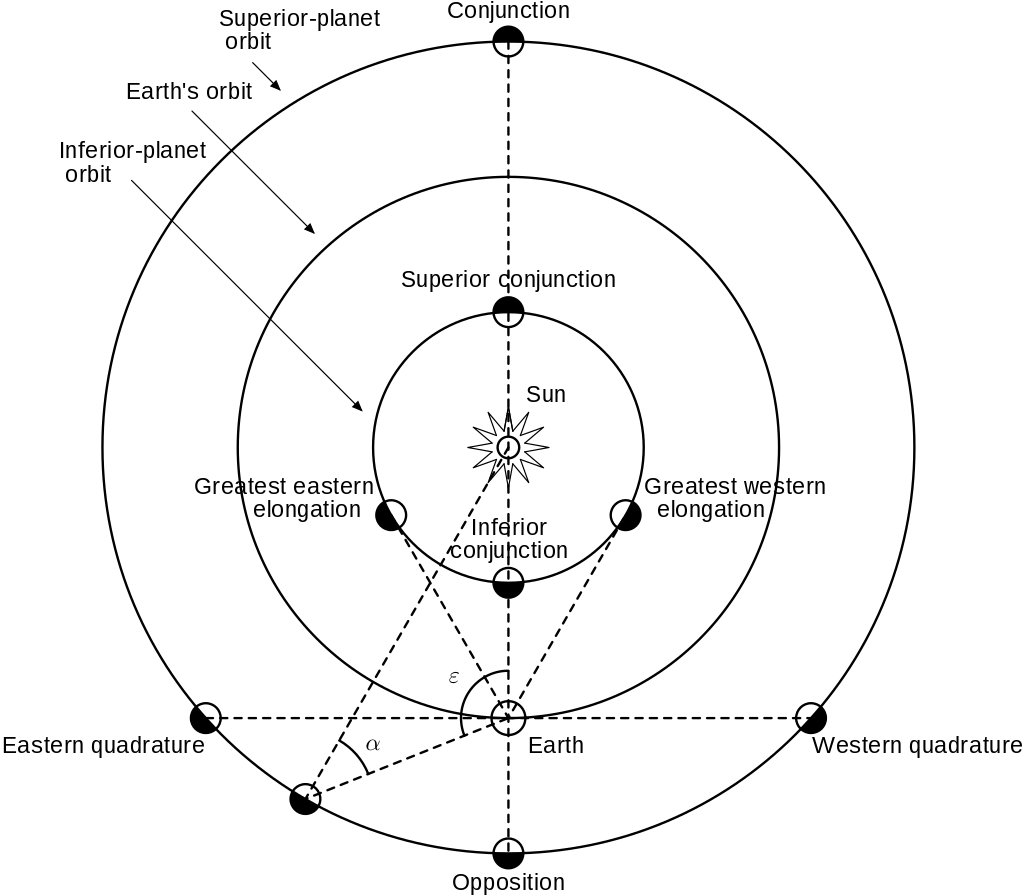
\includegraphics[width = 12cm]{report/Figures/methods/Positional_astronomy.png}
        \caption{Caption}
        \label{elongation}
    \end{figure}
    
    \begin{figure}[H]
        \centering
        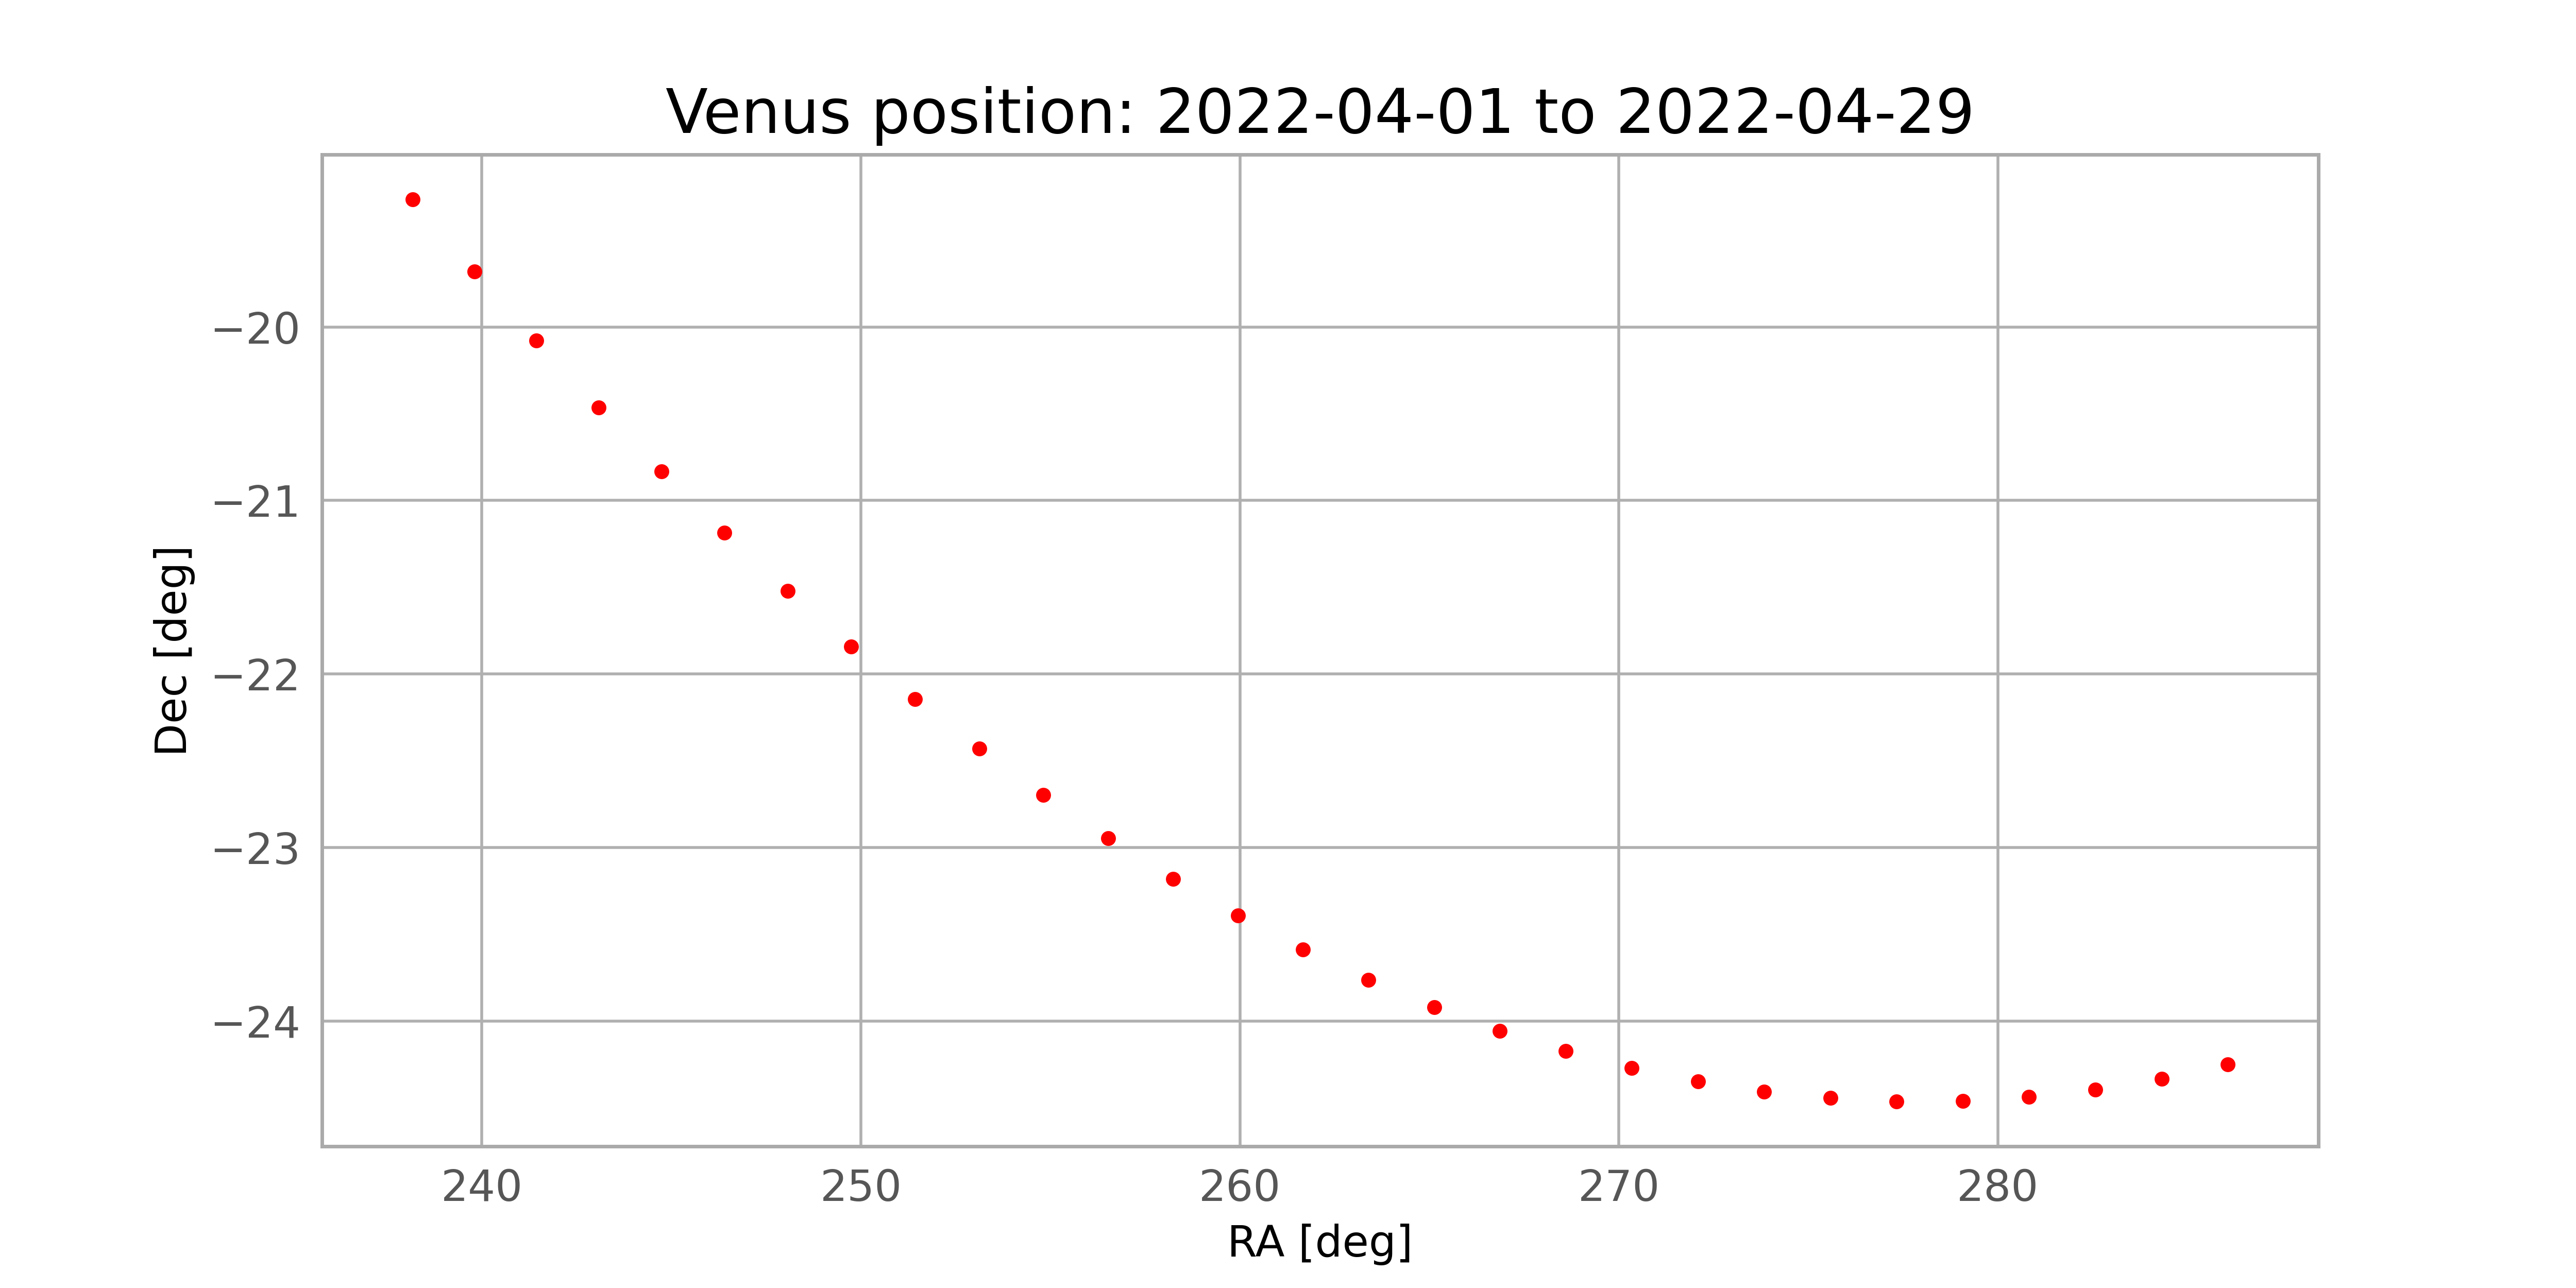
\includegraphics[width = 12cm]{report/Figures/methods/Venus_position.png}
        \caption{Caption}
        \label{venus_pos}
    \end{figure}
    
    %put here the different scw used
    \paragraph{22.04.2022 data}

    The April 22 data consists of...
    
    \textbf{Fig.} \ref{22_flux_map} shows ...
    
        \begin{figure}[H]
        \centering
        \begin{subfigure}{.3\textwidth}
            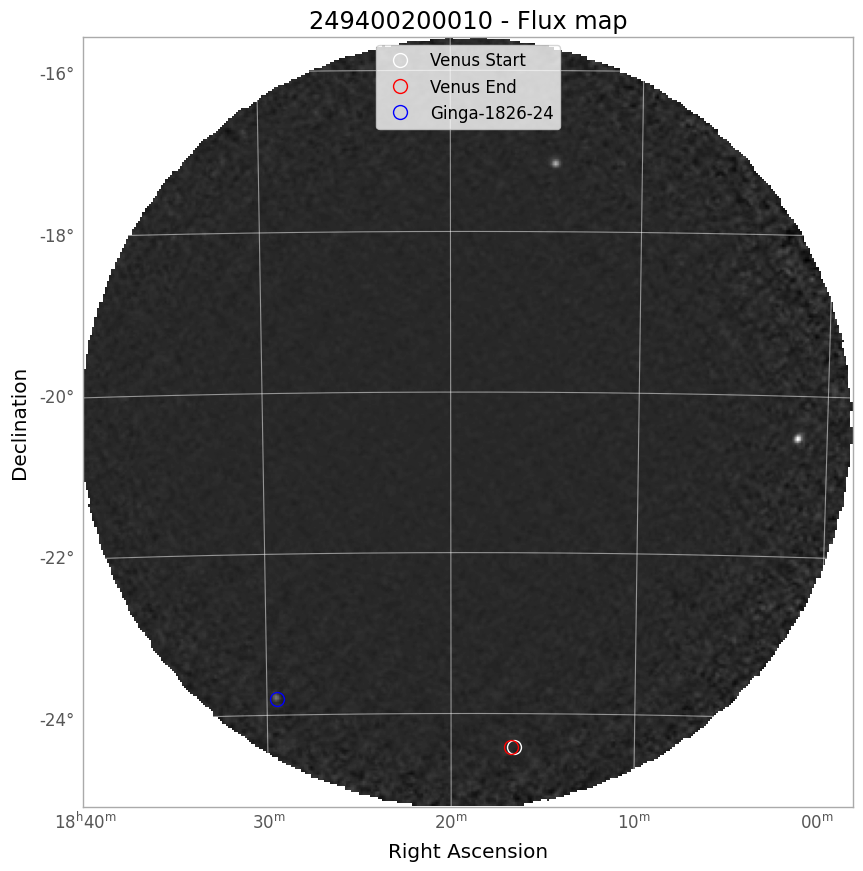
\includegraphics[width=\textwidth]{report/Figures/methods/2204/20_map.png}
        \end{subfigure}%
        \hspace{1em}-
        \begin{subfigure}{.3\textwidth}
            \centering
            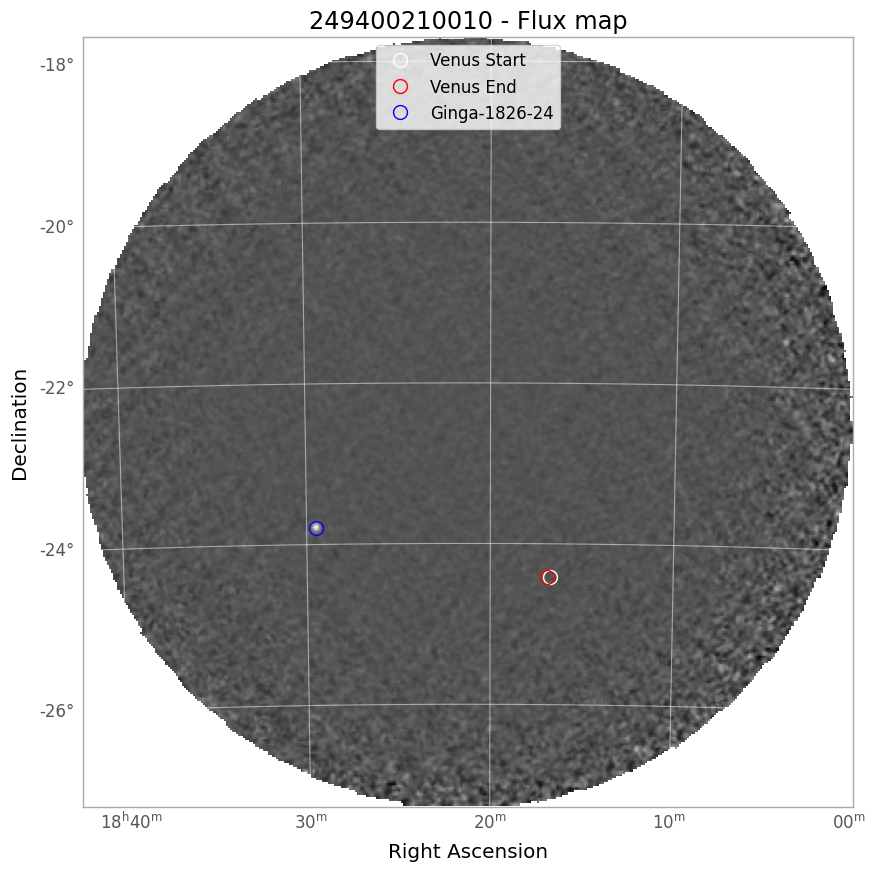
\includegraphics[width=\textwidth]{report/Figures/methods/2204/21_map.png}
        \end{subfigure}
        \hspace{1em}-
        \begin{subfigure}{.3\textwidth}
            \centering
            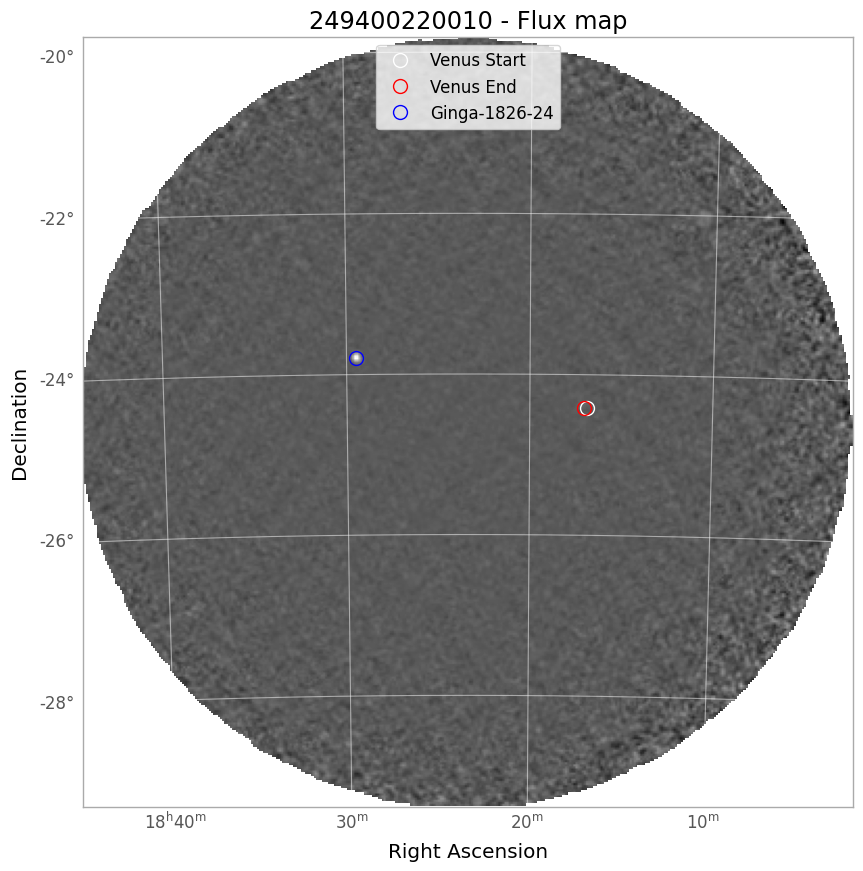
\includegraphics[width=\textwidth]{report/Figures/methods/2204/22_map.png}
        \end{subfigure}
        \hspace{1em}-
        \begin{subfigure}{.3\textwidth}
            \centering
            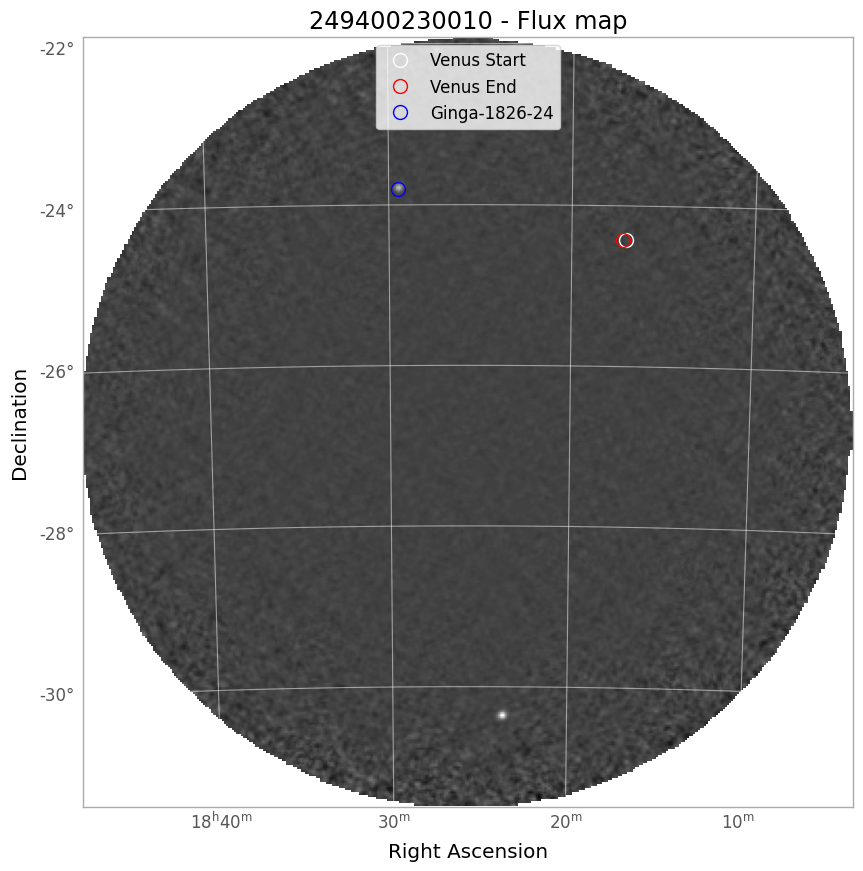
\includegraphics[width=\textwidth]{report/Figures/methods/2204/23_map.png}
        \end{subfigure}
        \hspace{1em}-
        \begin{subfigure}{.3\textwidth}
            \centering
            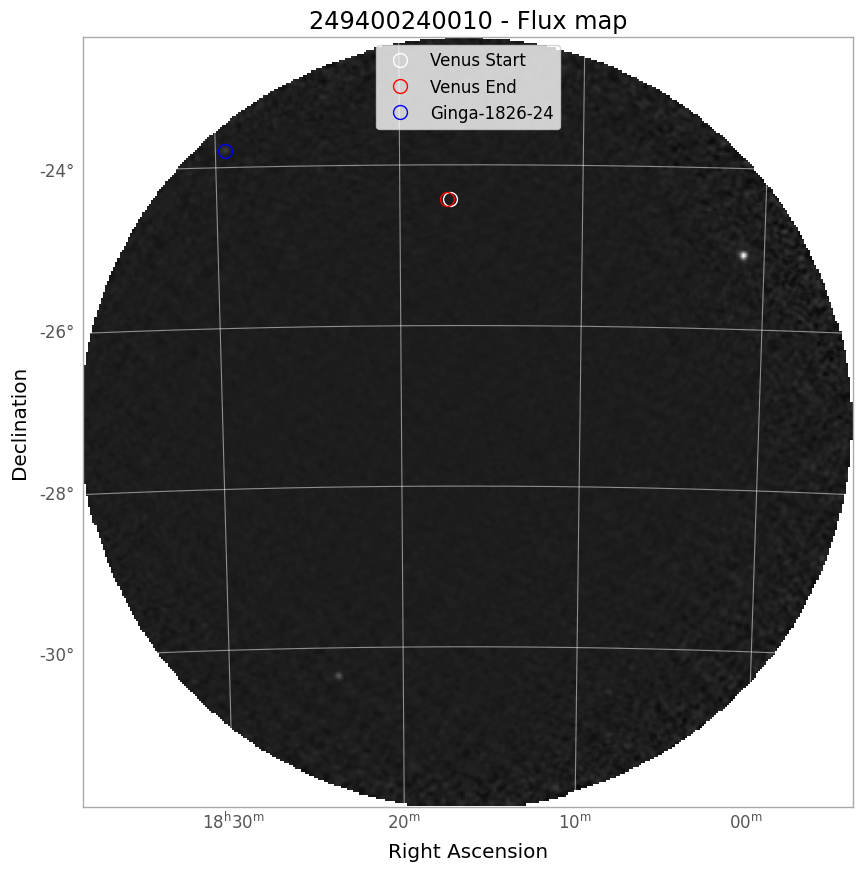
\includegraphics[width=\textwidth]{report/Figures/methods/2204/24_map.png}
        \end{subfigure}
        \hspace{1em}-
        \begin{subfigure}{.3\textwidth}
            \centering
            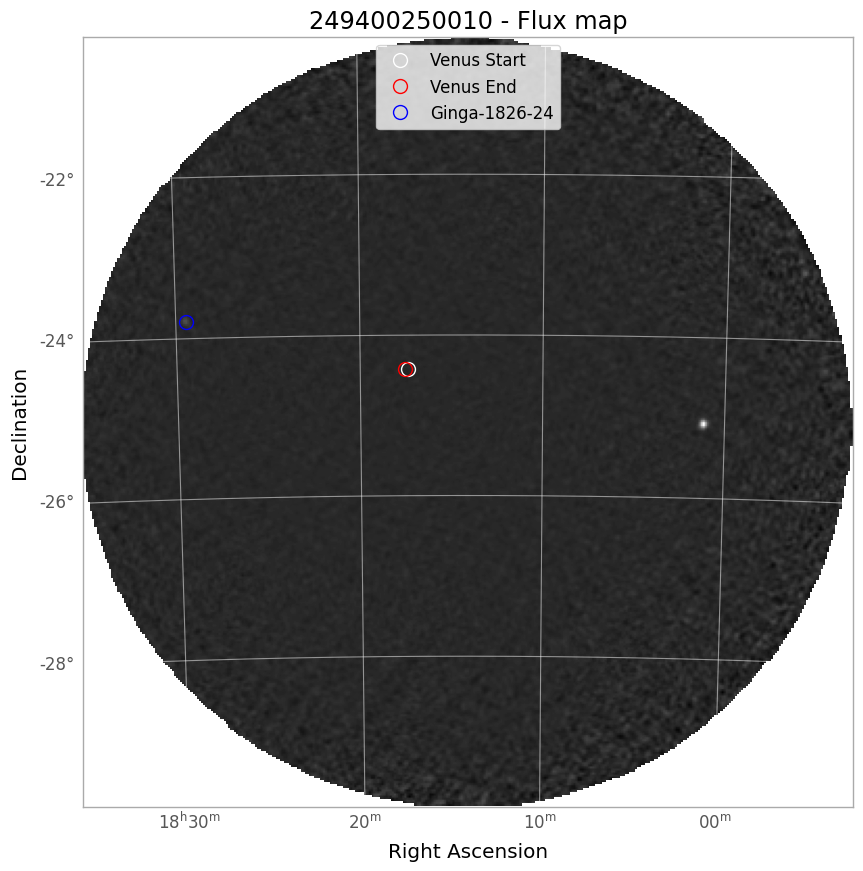
\includegraphics[width=\textwidth]{report/Figures/methods/2204/25_map.png}
        \end{subfigure}
        \hspace{1em}-
        \begin{subfigure}{.3\textwidth}
            \centering
            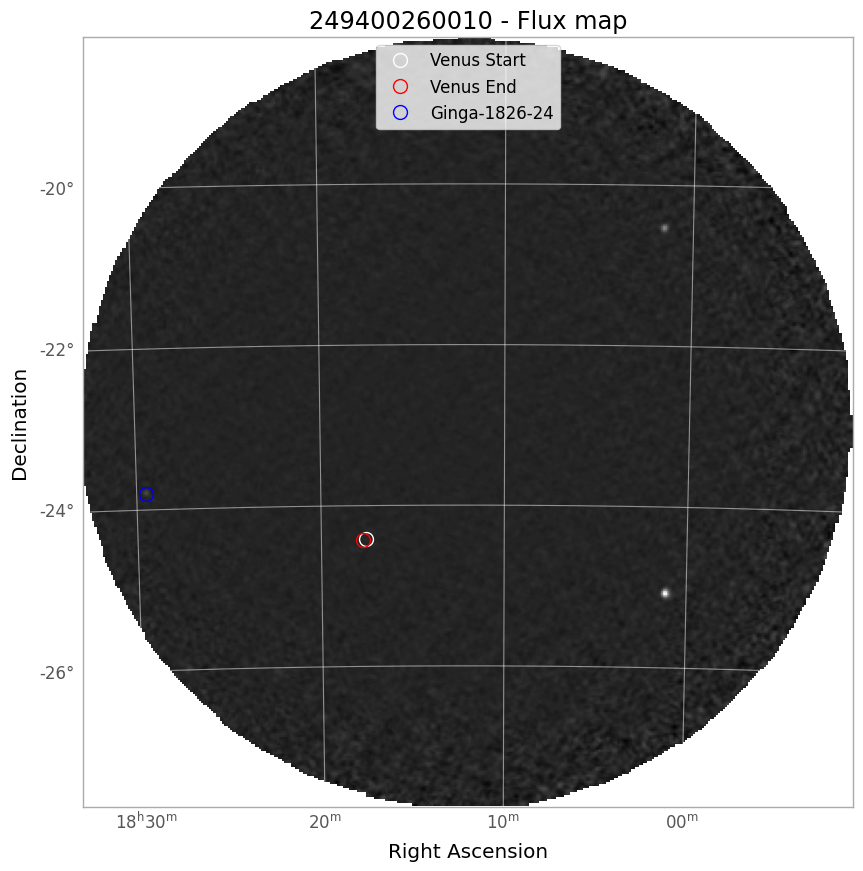
\includegraphics[width=\textwidth]{report/Figures/methods/2204/26_map.png}
        \end{subfigure}
        \hspace{1em}-
        \begin{subfigure}{.3\textwidth}
            \centering
            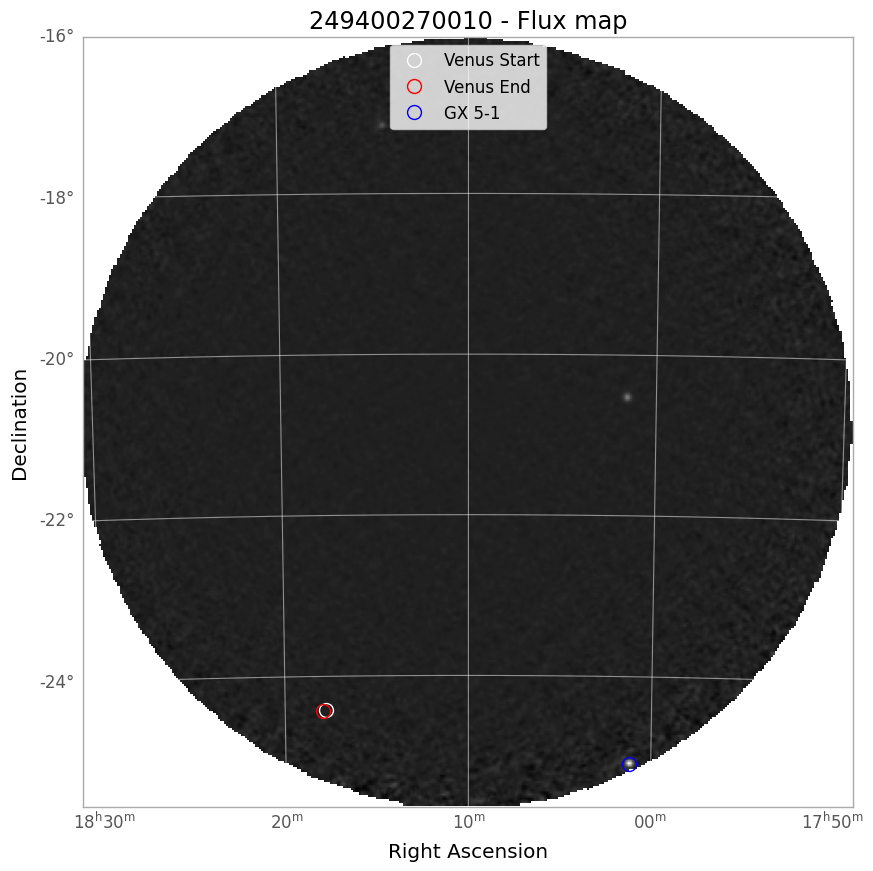
\includegraphics[width=\textwidth]{report/Figures/methods/2204/27_map.png}
        \end{subfigure}
        \hspace{1em}-
        \begin{subfigure}{.3\textwidth}
            \centering
            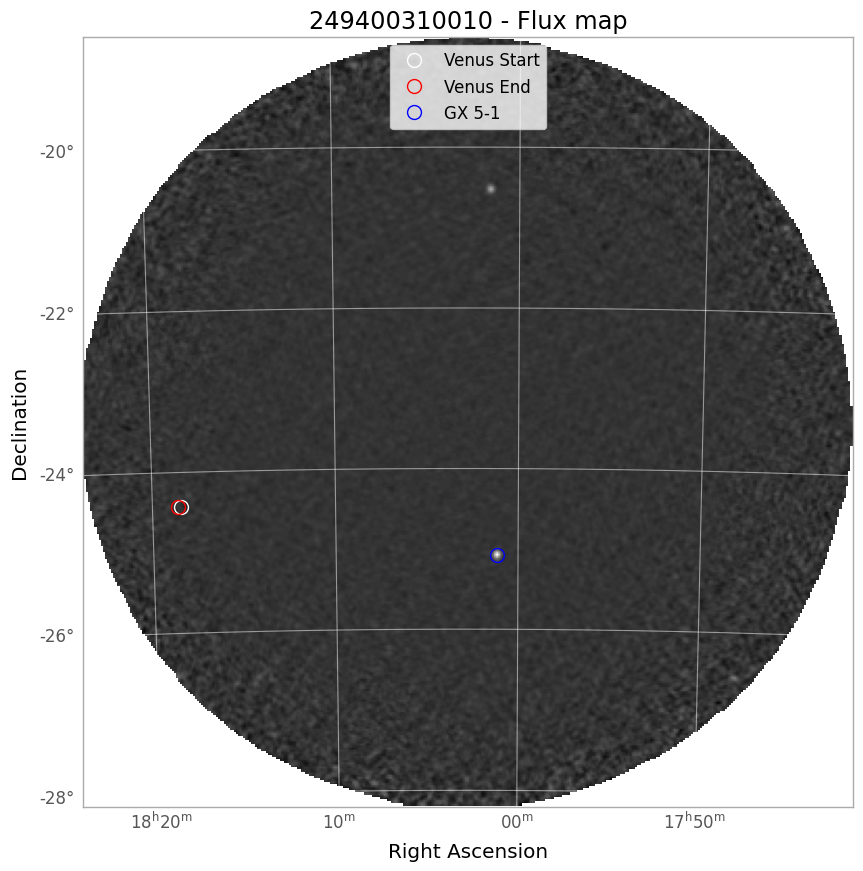
\includegraphics[width=\textwidth]{report/Figures/methods/2204/31_map.png}
        \end{subfigure}
        \hspace{1em}-
        \begin{subfigure}{.3\textwidth}
            \centering
            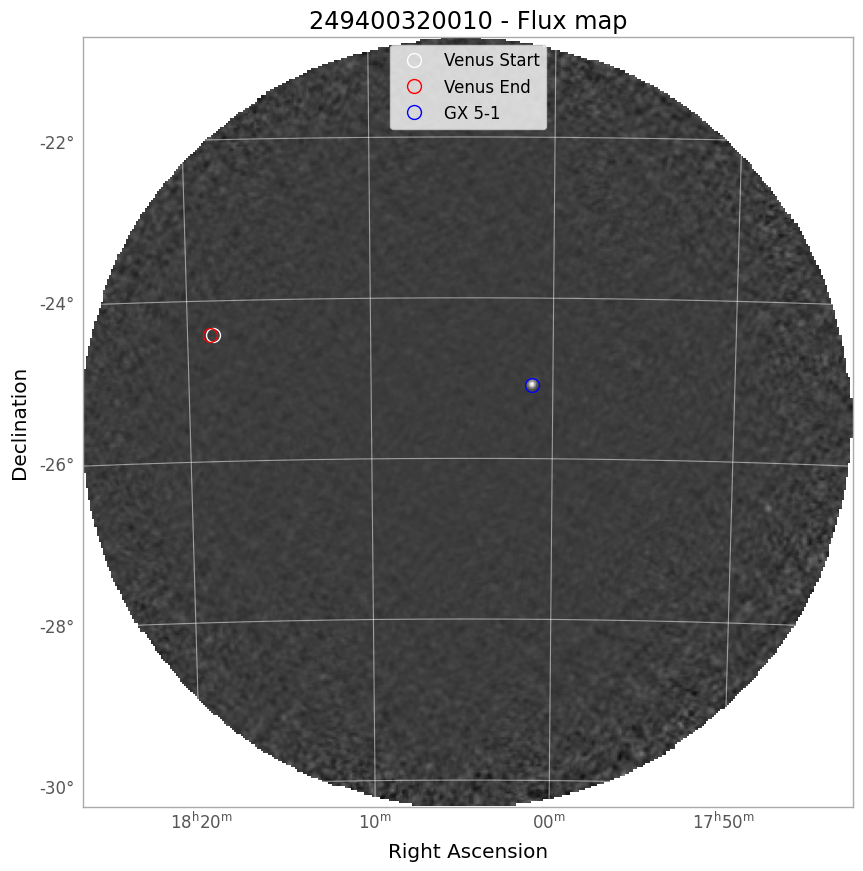
\includegraphics[width=\textwidth]{report/Figures/methods/2204/32_map.png}
        \end{subfigure}
        \hspace{1em}-
        \begin{subfigure}{.3\textwidth}
            \centering
            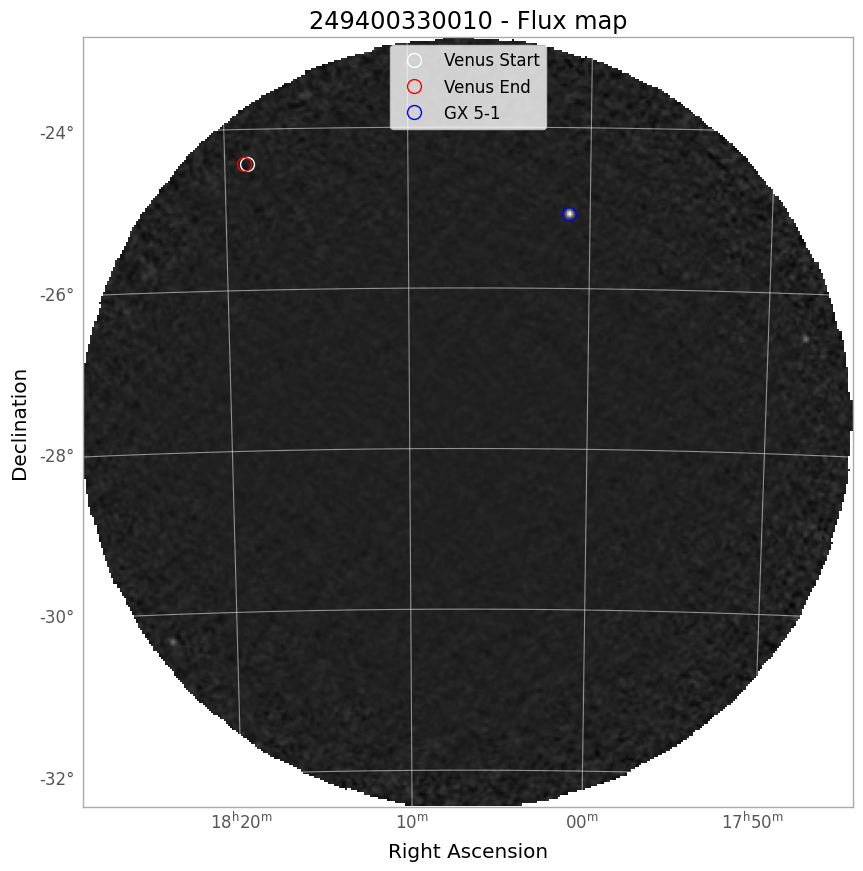
\includegraphics[width=\textwidth]{report/Figures/methods/2204/33_map.png}
        \end{subfigure}
        \caption{}
        \label{22_flux_map}
        \end{figure}

        \begin{figure}[H]
        \centering
        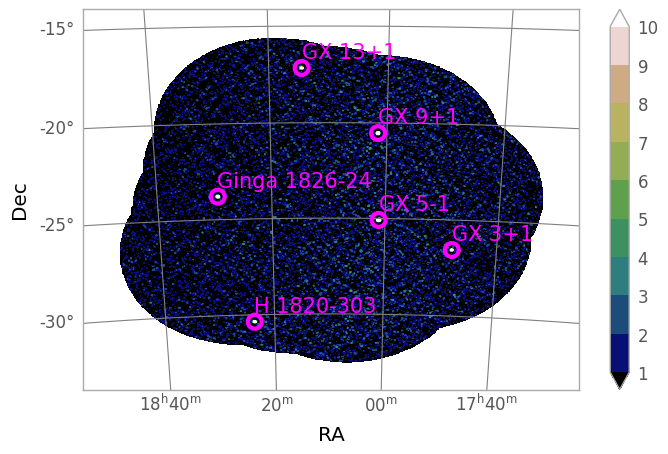
\includegraphics[width = 12cm]{report/Figures/methods/2204/oda_2204.png}
        \caption{Caption}
        \label{22_mosaic}
        \end{figure}
    
    \paragraph{24.04.2022 data}
    The April 24 data consists of ...

    \begin{figure}[H]
        \centering
        \begin{subfigure}{.45\textwidth}
            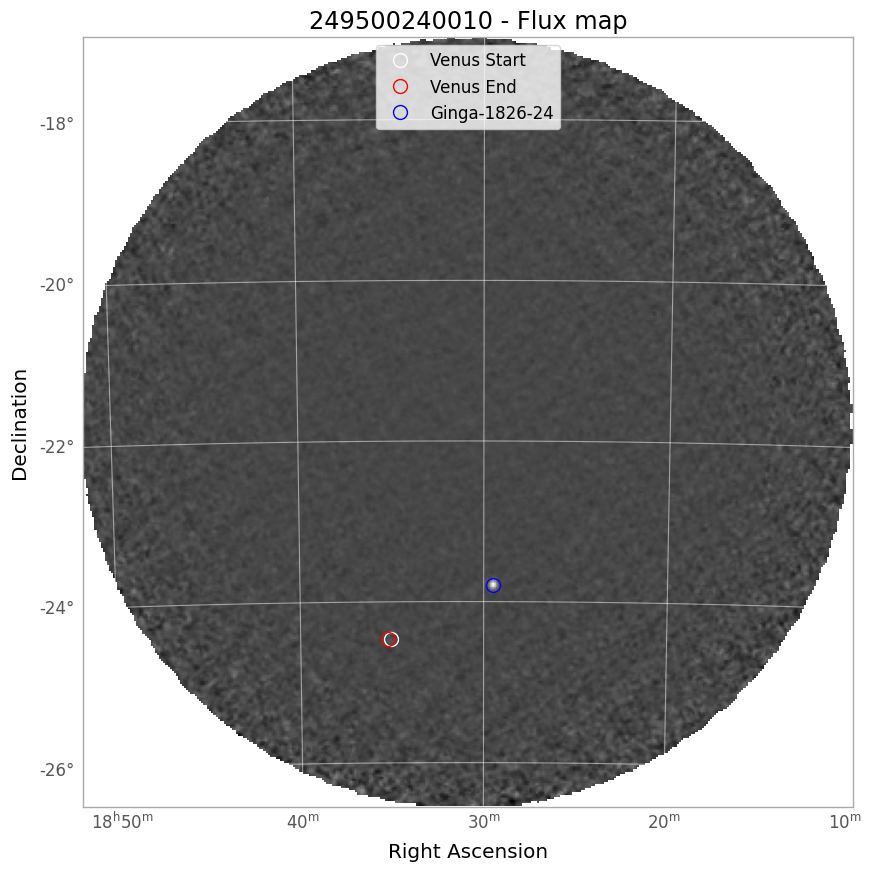
\includegraphics[width=\textwidth]{report/Figures/methods/2404/24_map.png}
        \end{subfigure}%
        \hspace{1em}-
        \begin{subfigure}{.45\textwidth}
            \centering
            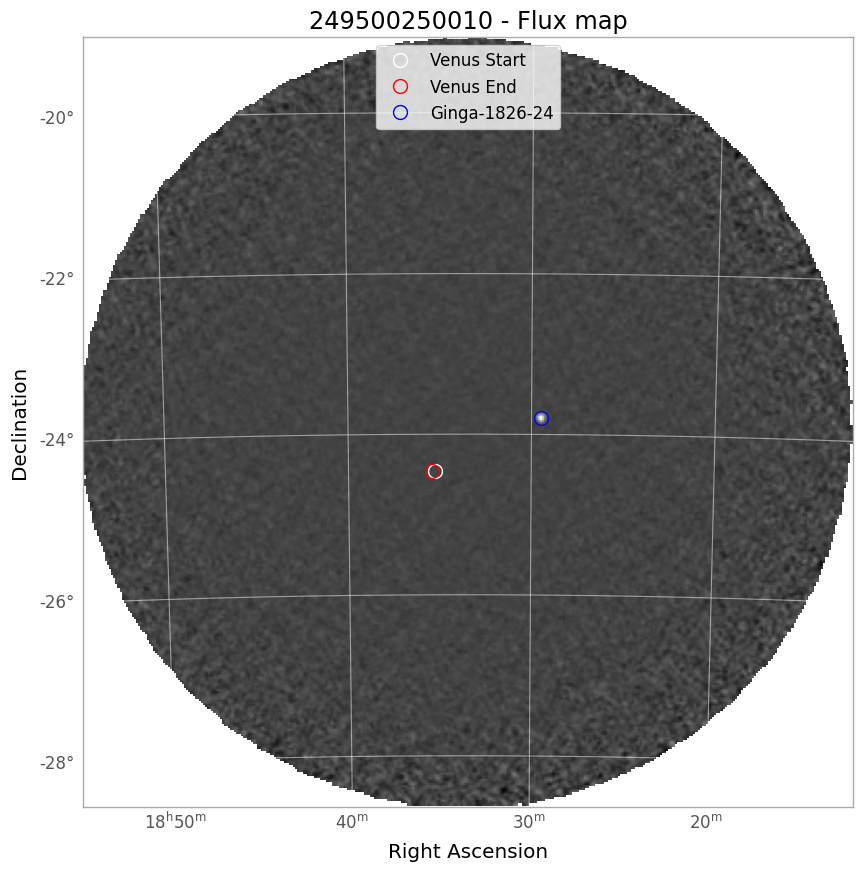
\includegraphics[width=\textwidth]{report/Figures/methods/2404/25_map.png}
        \end{subfigure}
        \hspace{1em}-
        \begin{subfigure}{.45\textwidth}
            \centering
            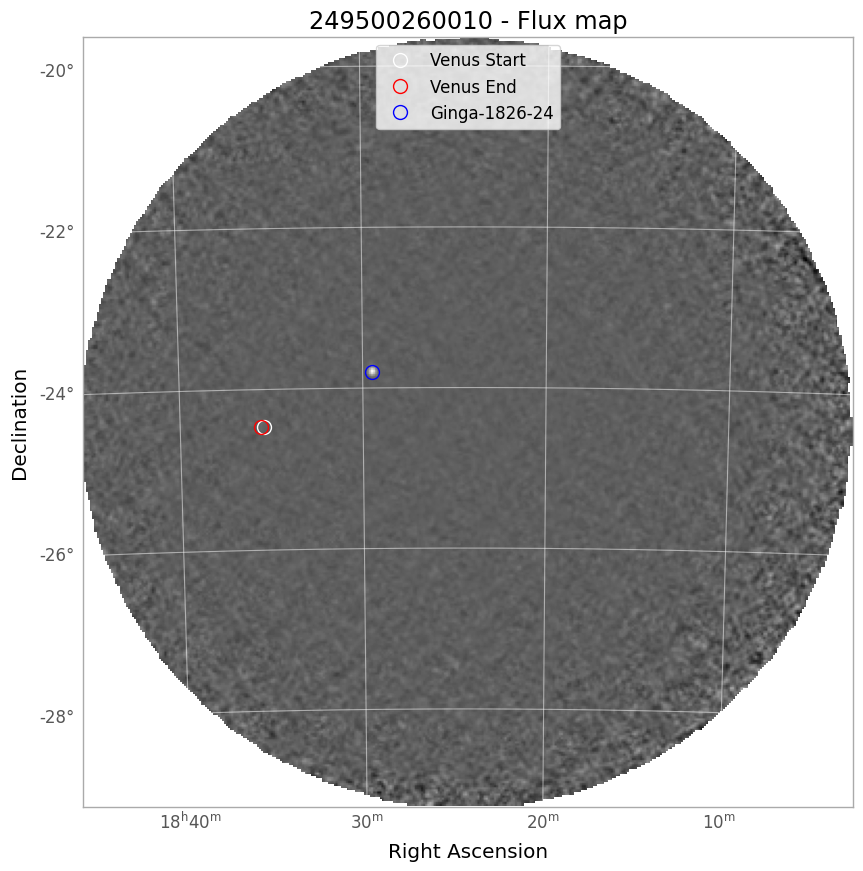
\includegraphics[width=\textwidth]{report/Figures/methods/2404/26_map.png}
        \end{subfigure}
        \hspace{1em}-
        \begin{subfigure}{.45\textwidth}
            \centering
            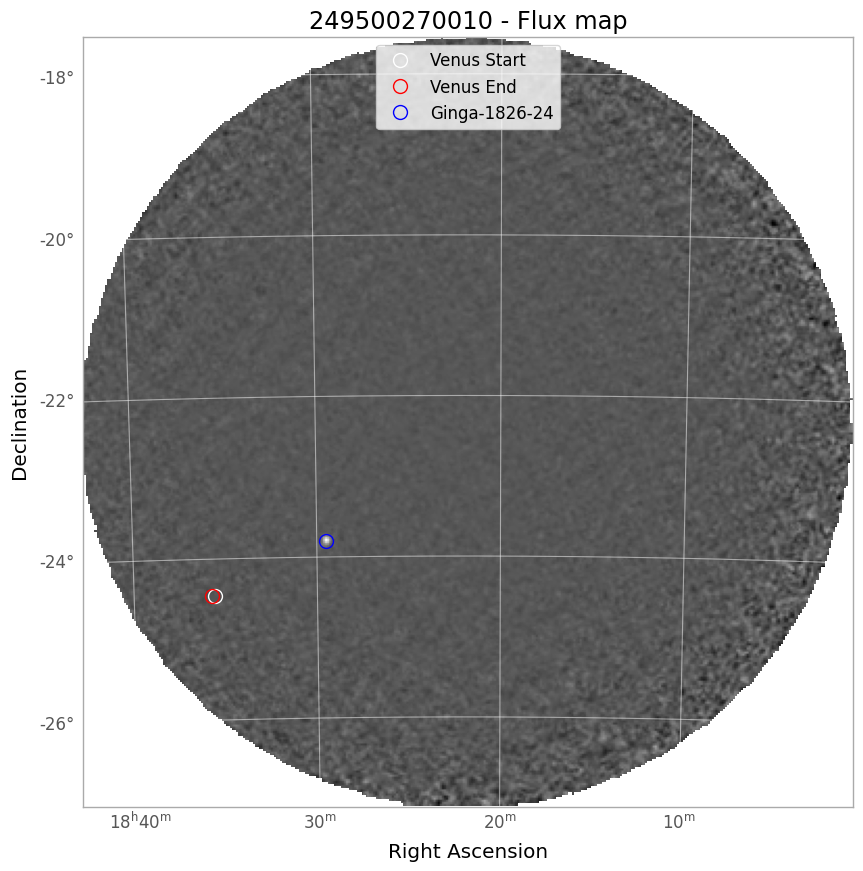
\includegraphics[width=\textwidth]{report/Figures/methods/2404/27_map.png}
        \end{subfigure}
        \caption{}
        \label{24_map}
    \end{figure}

        \begin{figure}[H]
        \centering
        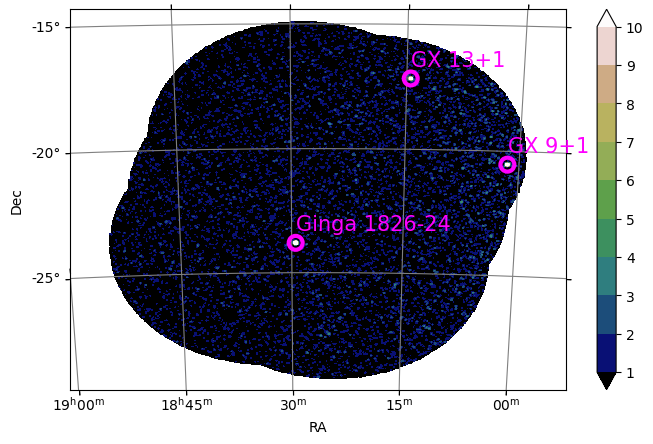
\includegraphics[width = 12cm]{report/Figures/methods/2404/oda_2404.png}
        \caption{Caption}
        \label{24_mosaic}
        \end{figure}

    
    \subsection{Models and assumptions}

        \begin{figure}[H]
        \centering
        \begin{subfigure}{.45\textwidth}
            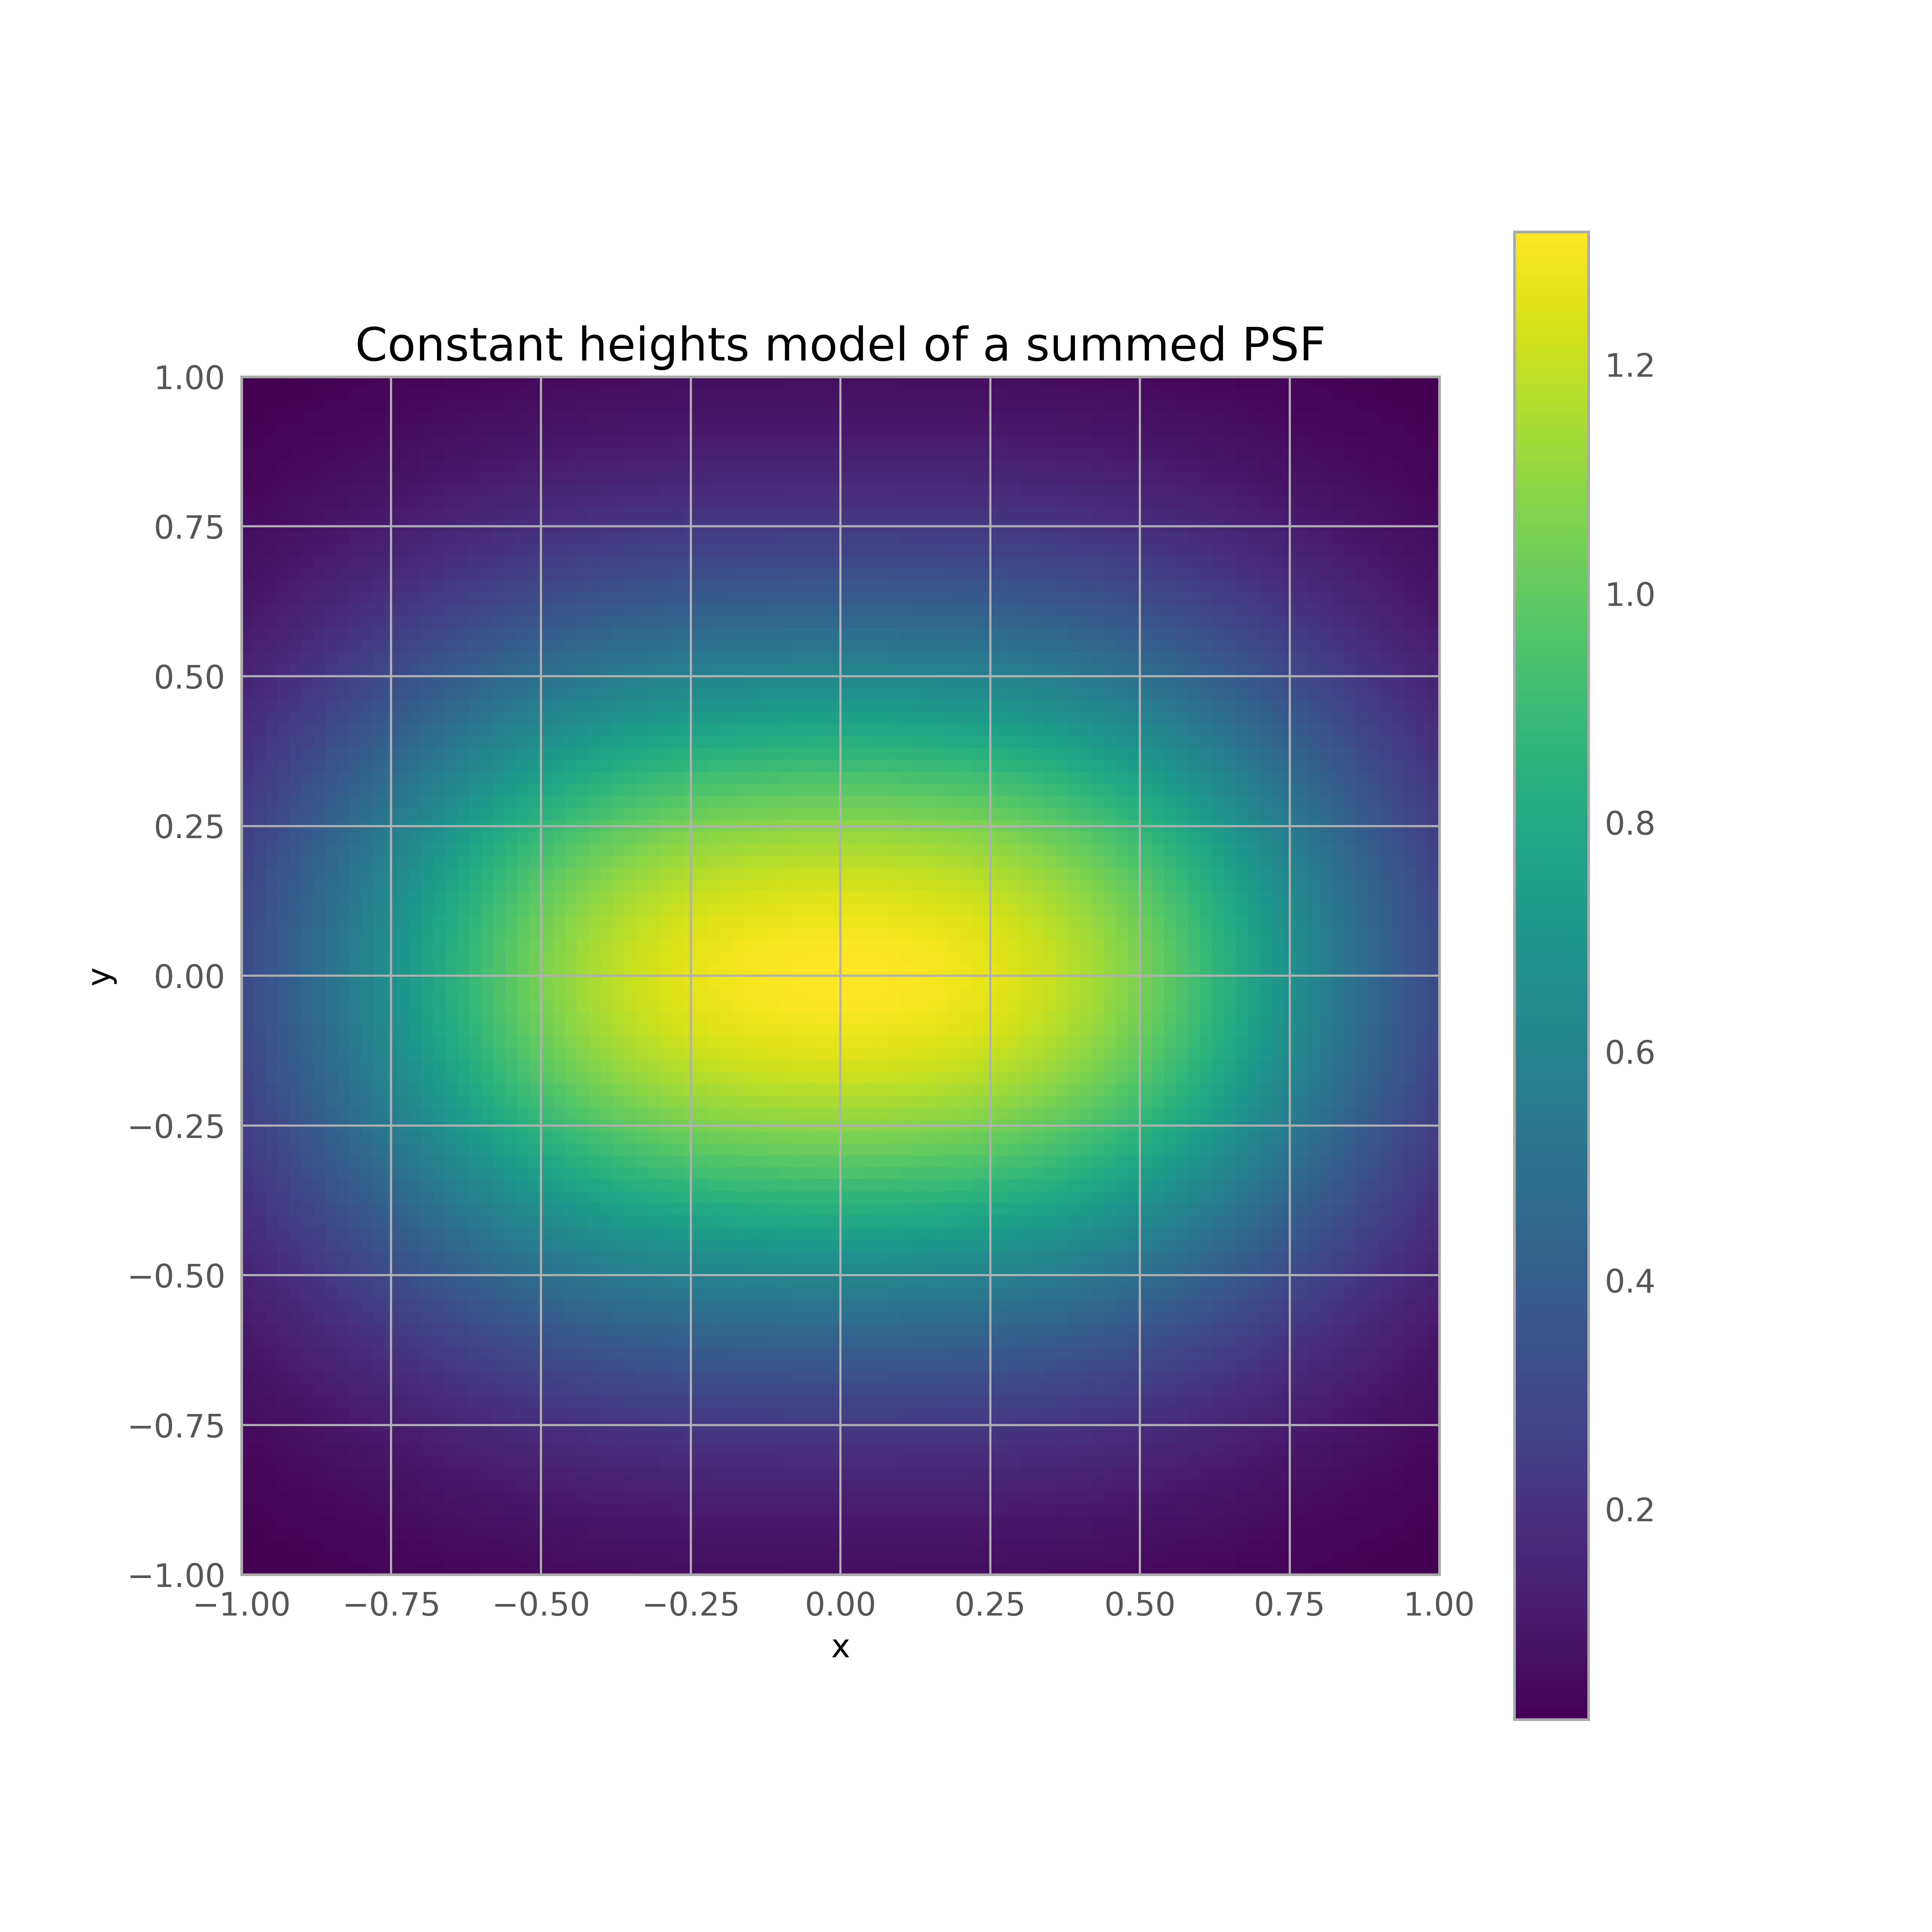
\includegraphics[width=\textwidth]{report/Figures/models/model_psf_const.png}
        \end{subfigure}%
        \hspace{1em}-
        \begin{subfigure}{.45\textwidth}
            \centering
            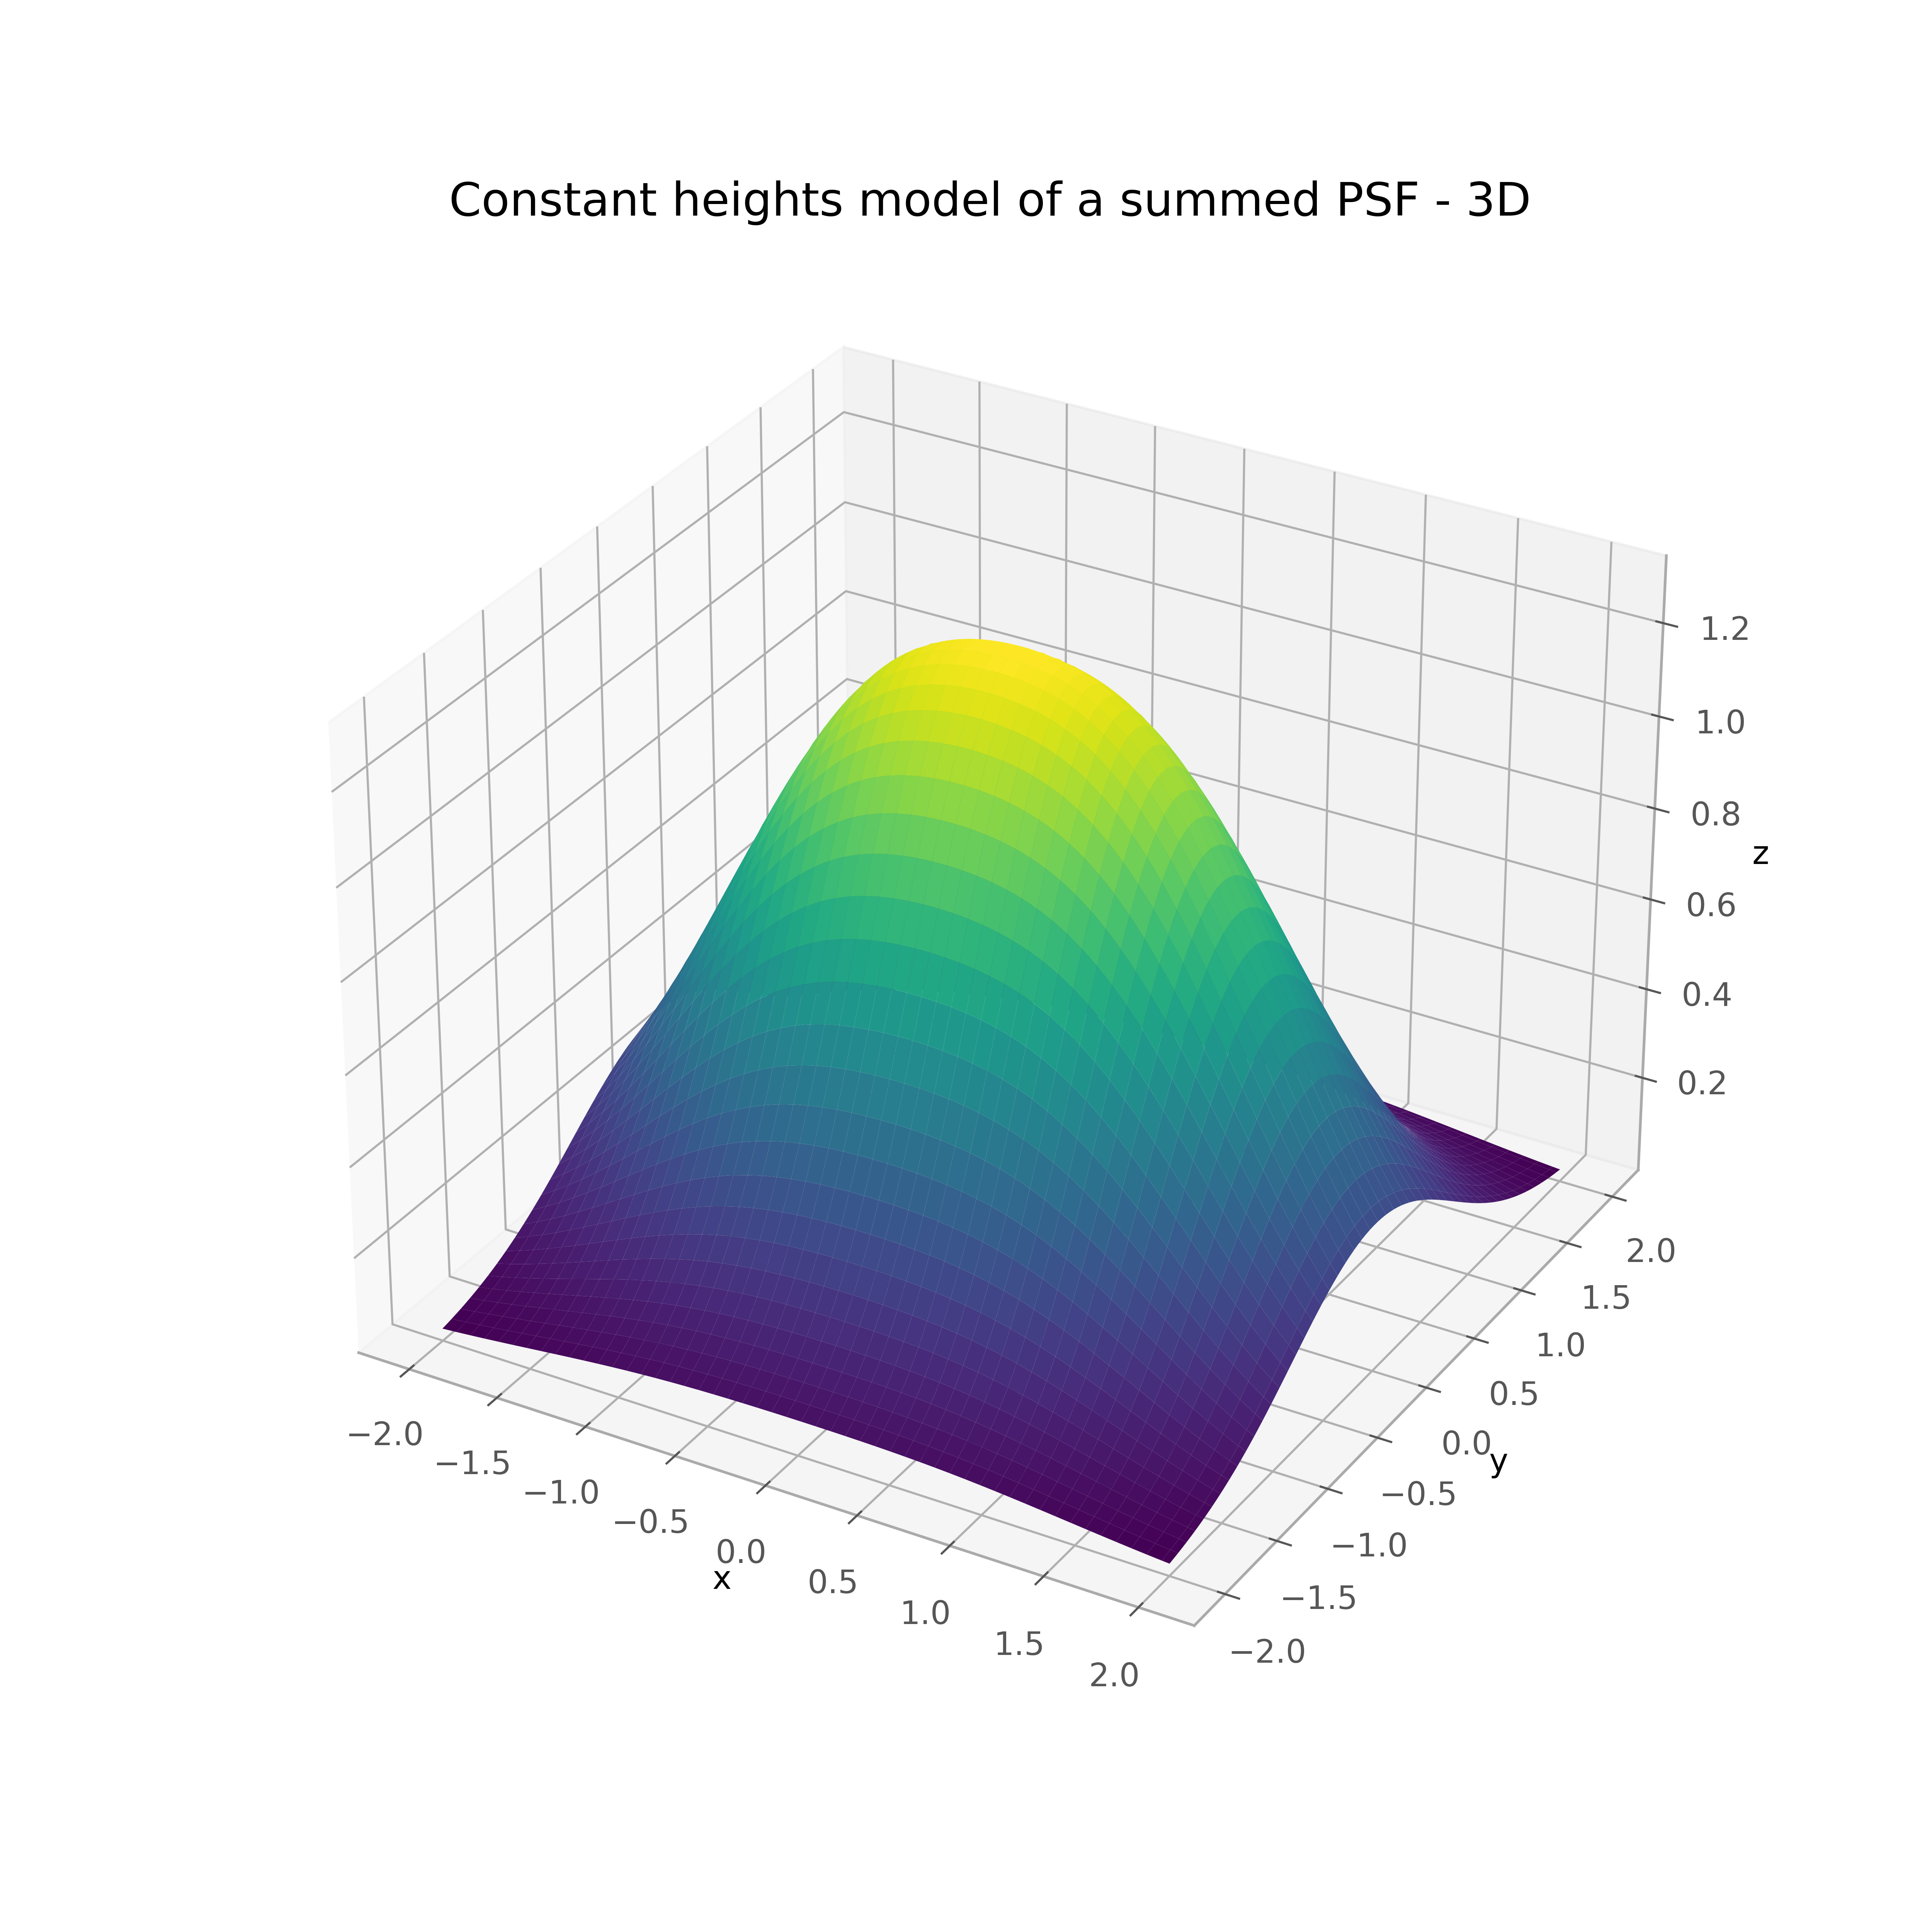
\includegraphics[width=\textwidth]{report/Figures/models/model_psf_const_3d.png}
        \end{subfigure}
        \caption{}
        \label{model_psf_const}
        \end{figure}

        \begin{figure}[H]
        \centering
        \begin{subfigure}{.45\textwidth}
            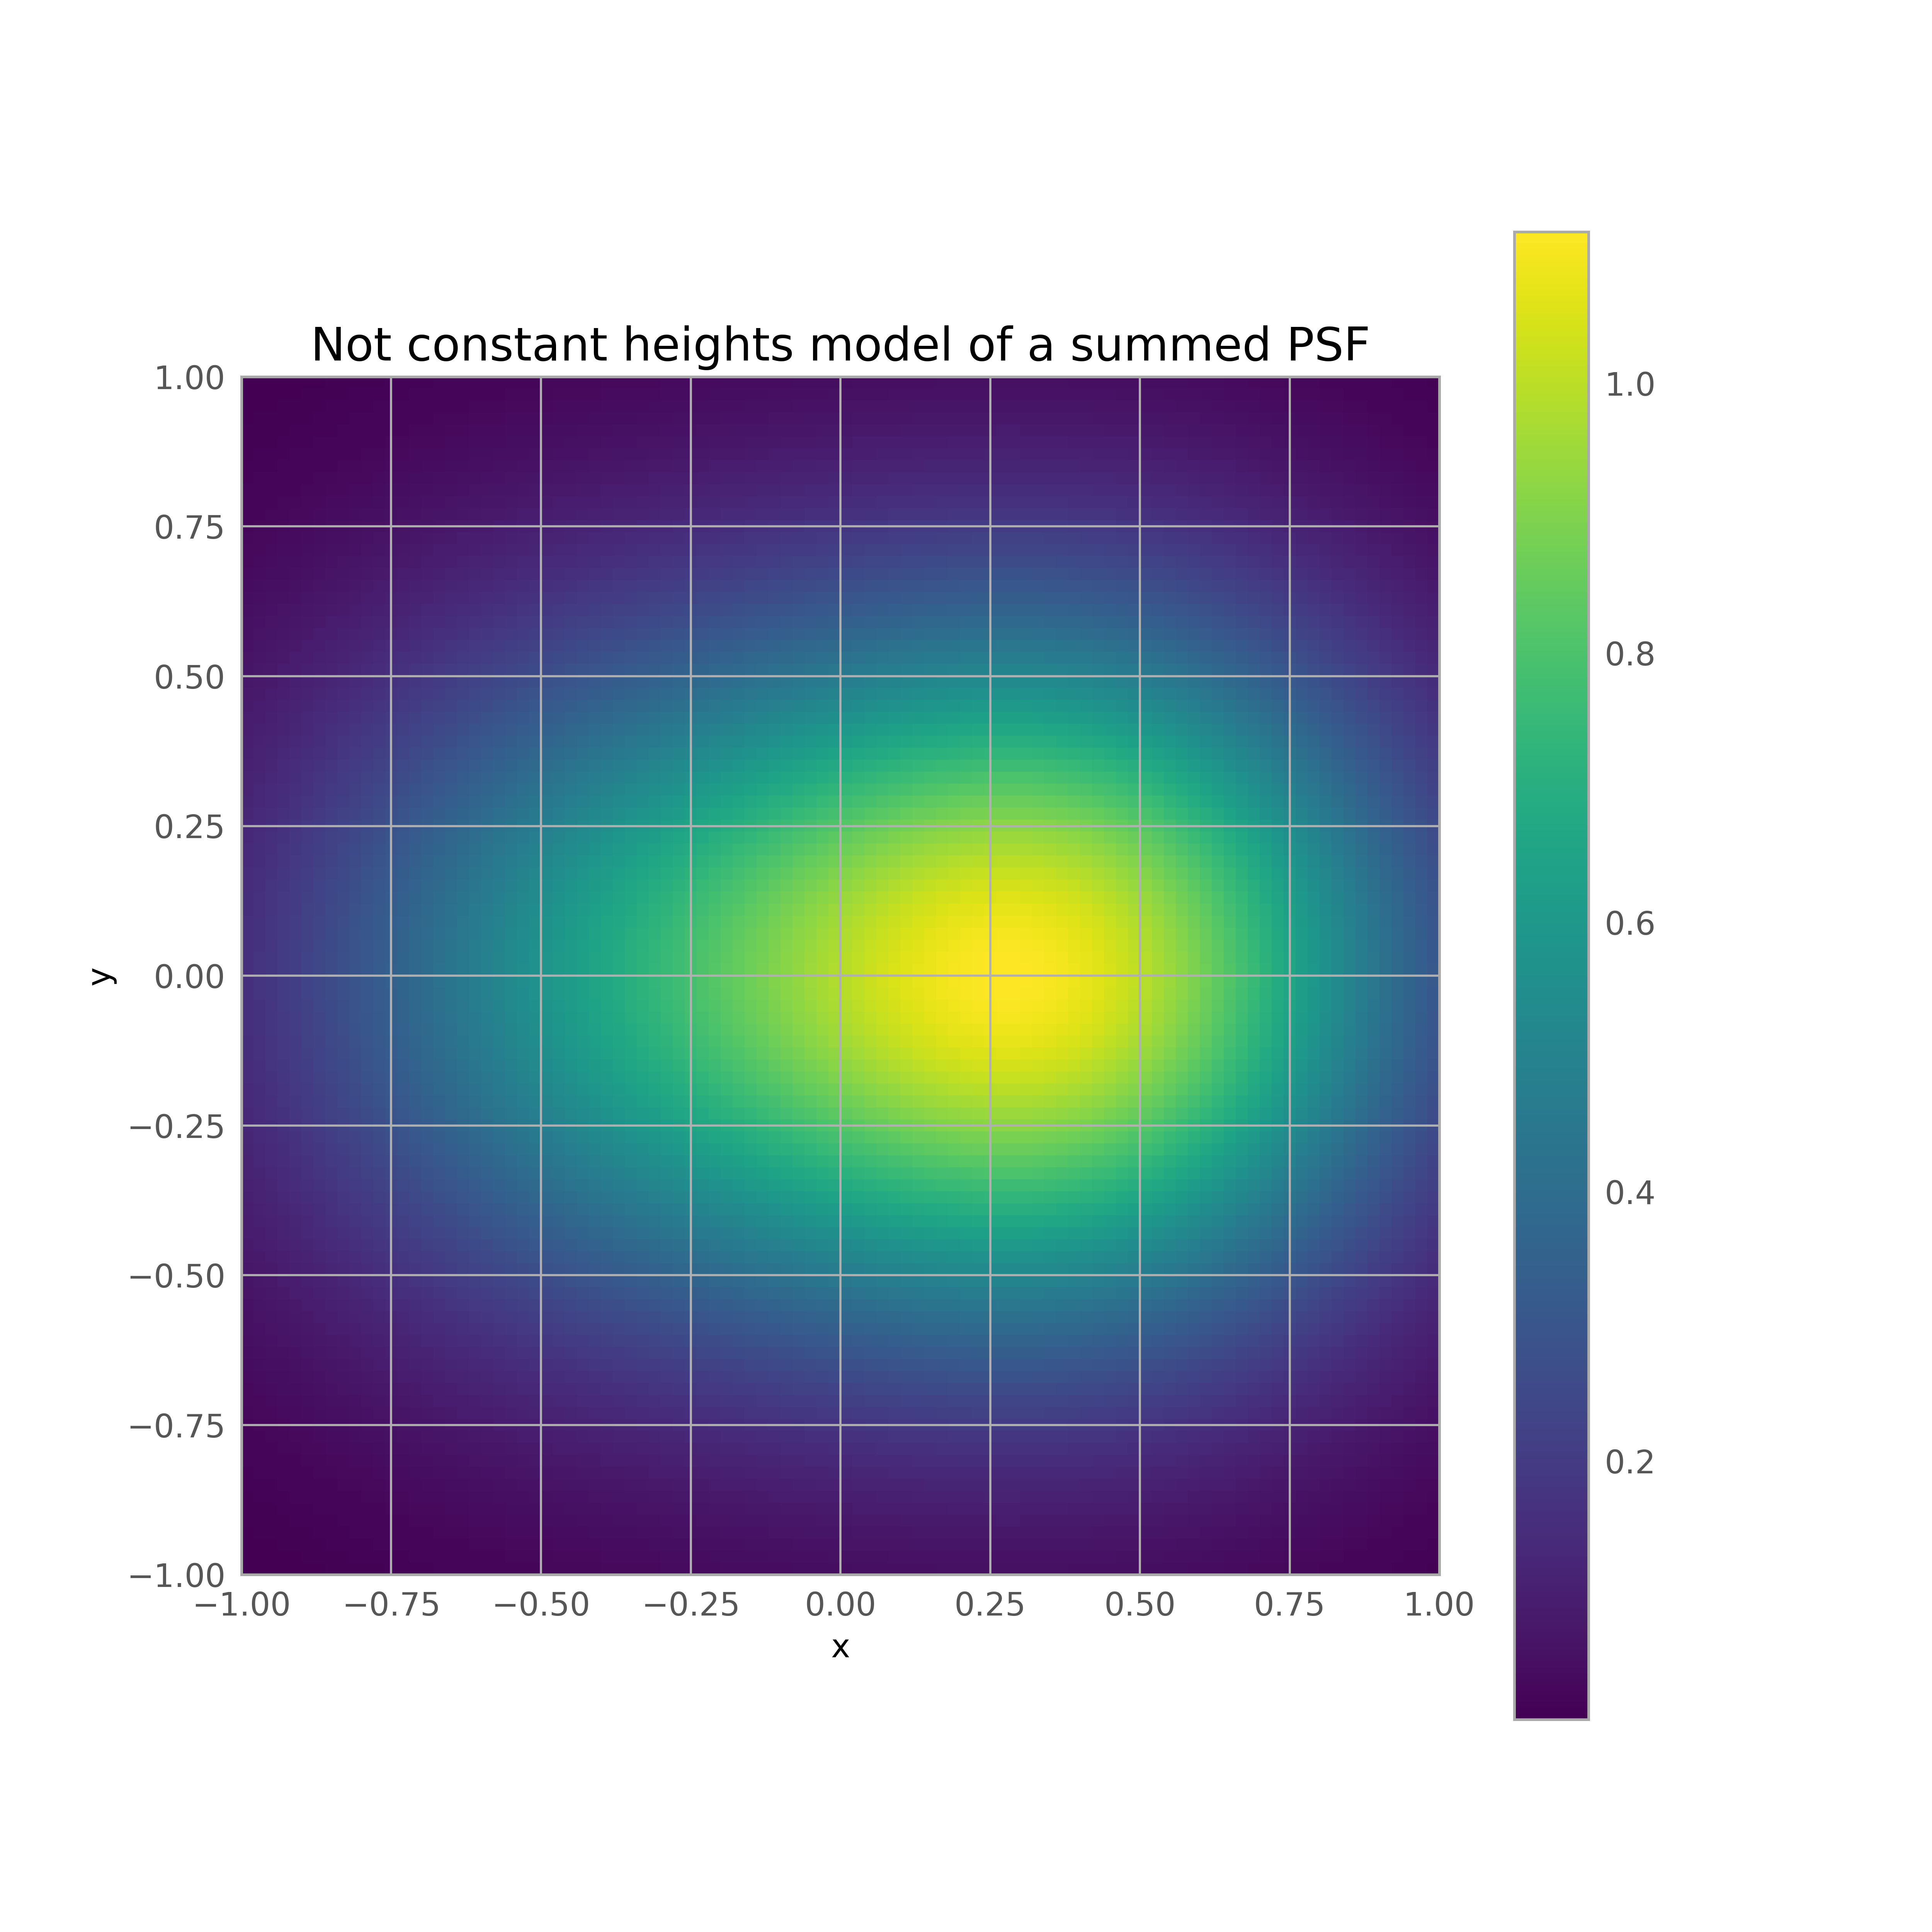
\includegraphics[width=\textwidth]{report/Figures/models/model_psf_notconst.png}
        \end{subfigure}%
        \hspace{1em}-
        \begin{subfigure}{.45\textwidth}
            \centering
            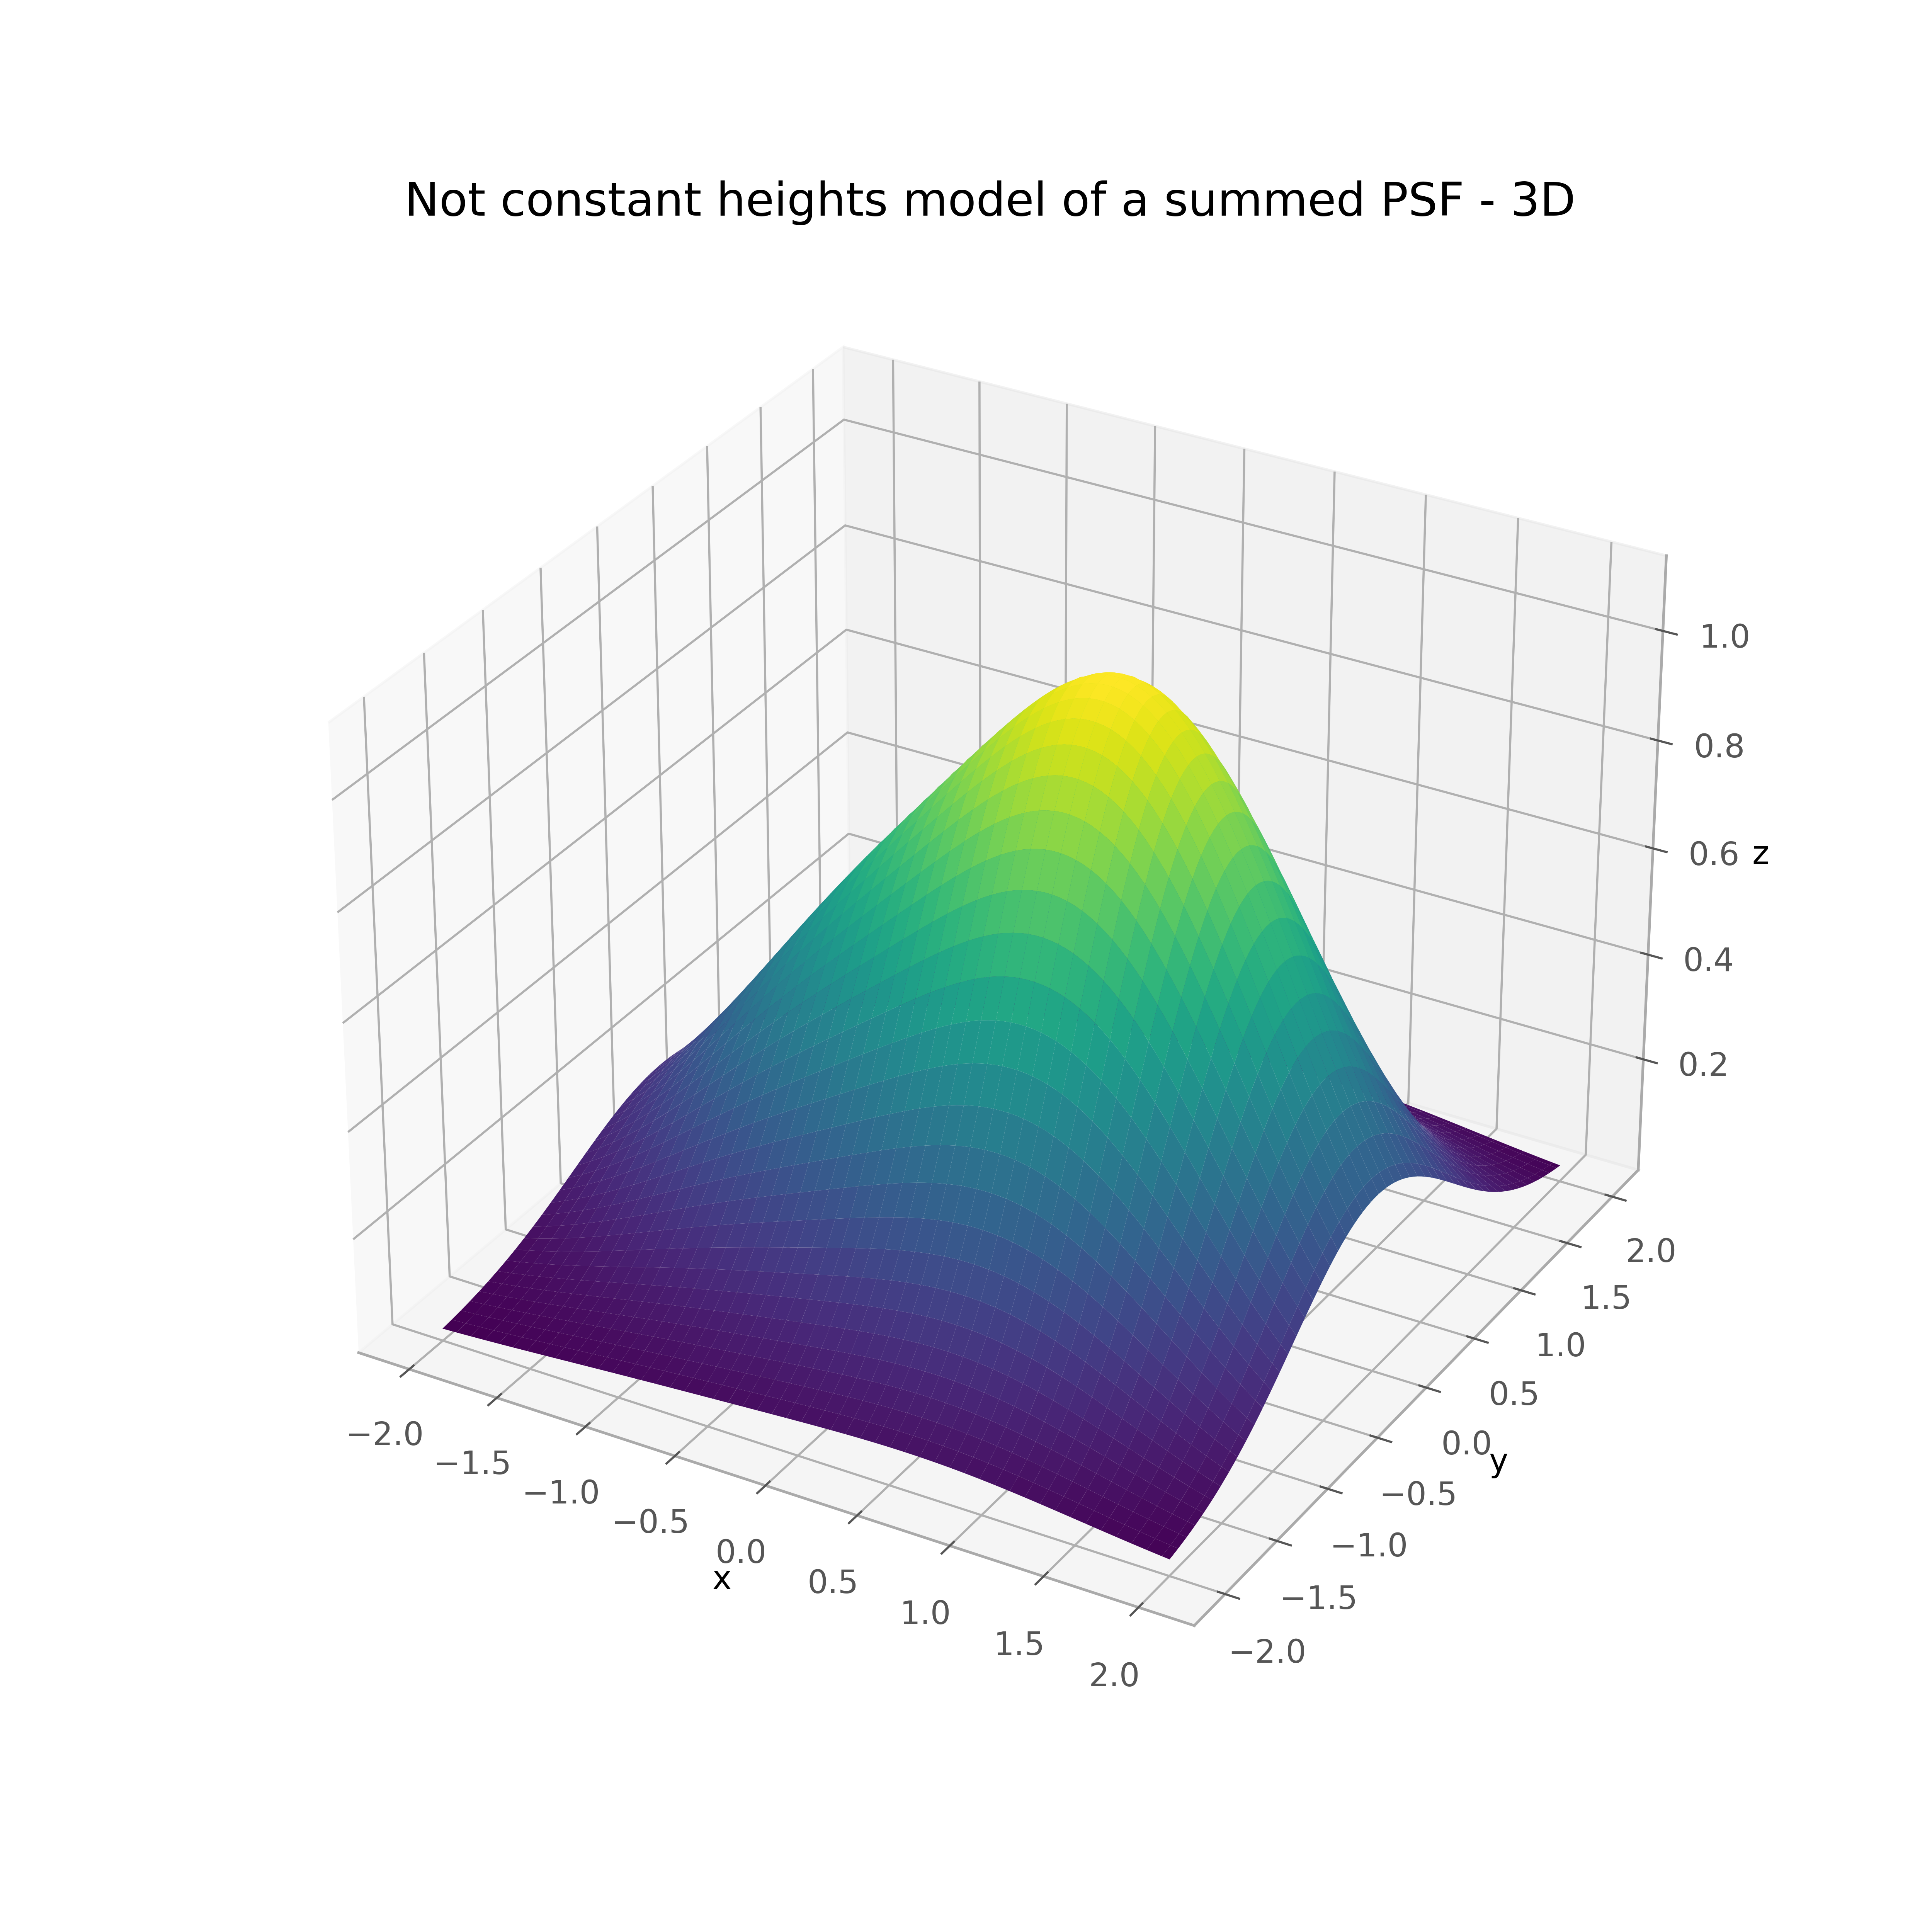
\includegraphics[width=\textwidth]{report/Figures/models/model_psf_notconst_3d.png}
        \end{subfigure}
        \caption{}
        \label{model_psf_notconst}
        \end{figure}

        \begin{figure}[H]
        \centering
        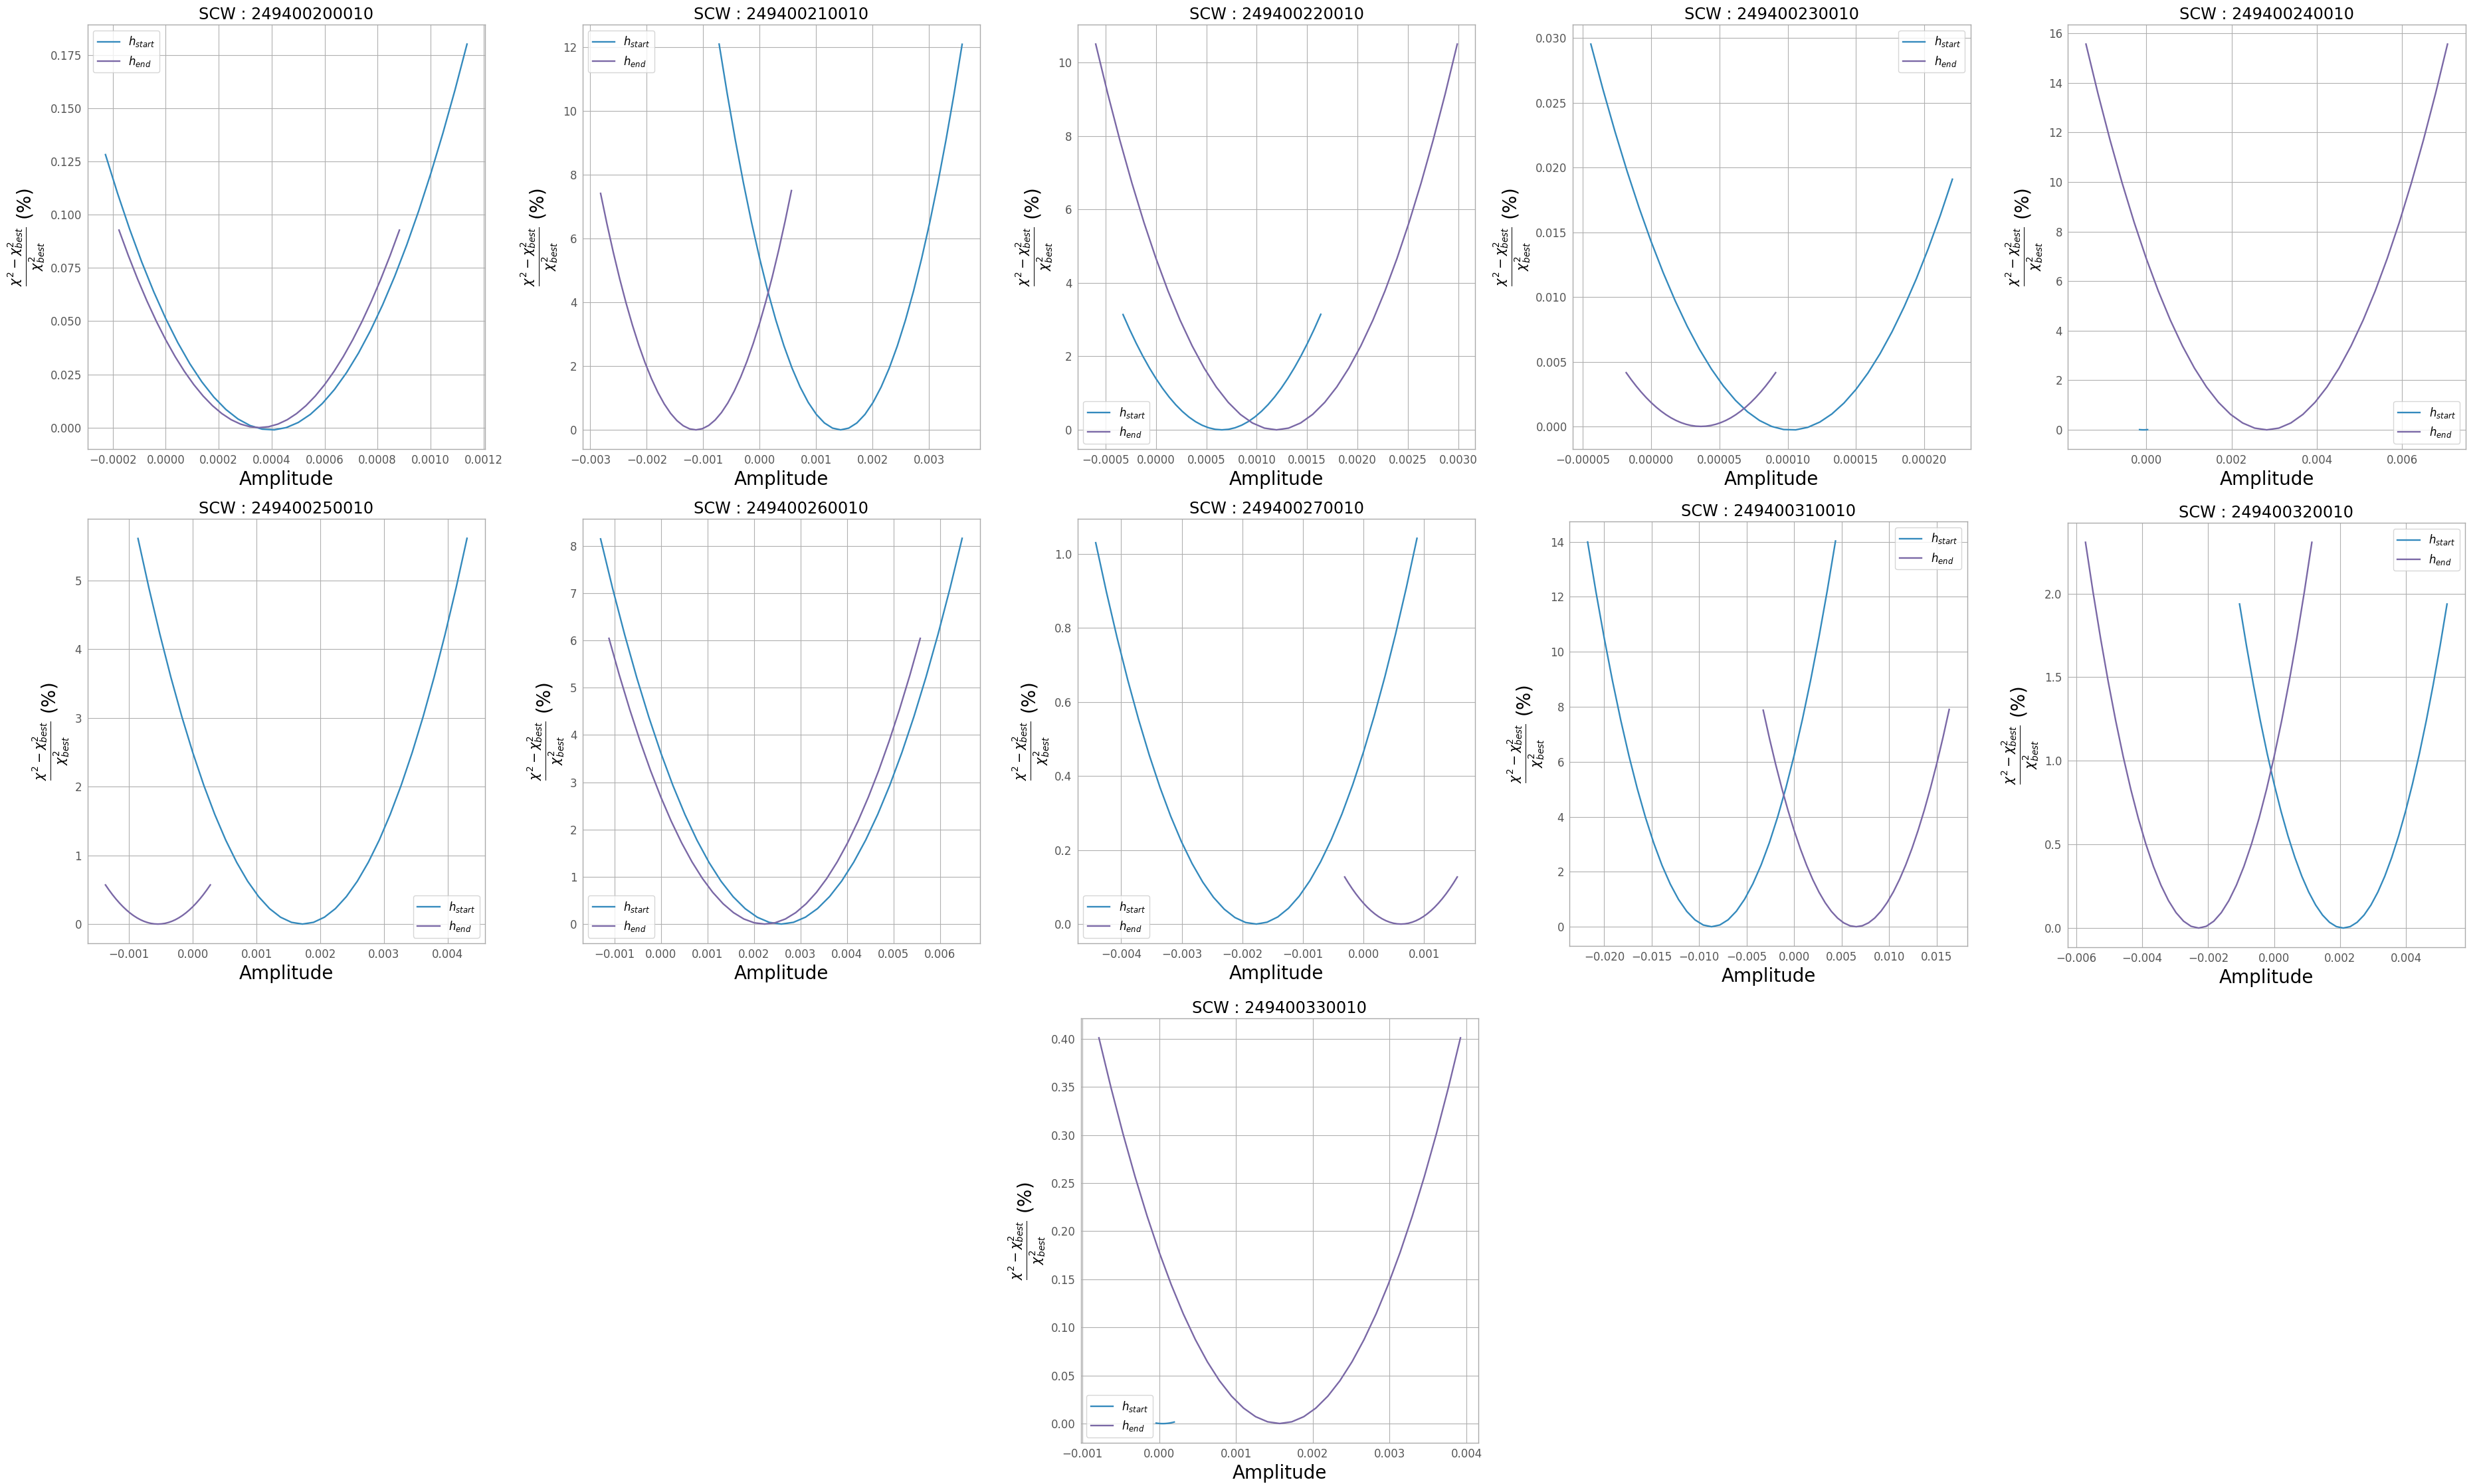
\includegraphics[width = \textwidth]{report/Figures/models/2204/threshold_determination_notconst.png}
        \caption{Caption}
        \label{threshold}
        \end{figure}

    
    %--------------------------------------------------
    
    \subsection{Solar events}
    
    \begin{figure}[H]
        \centering
        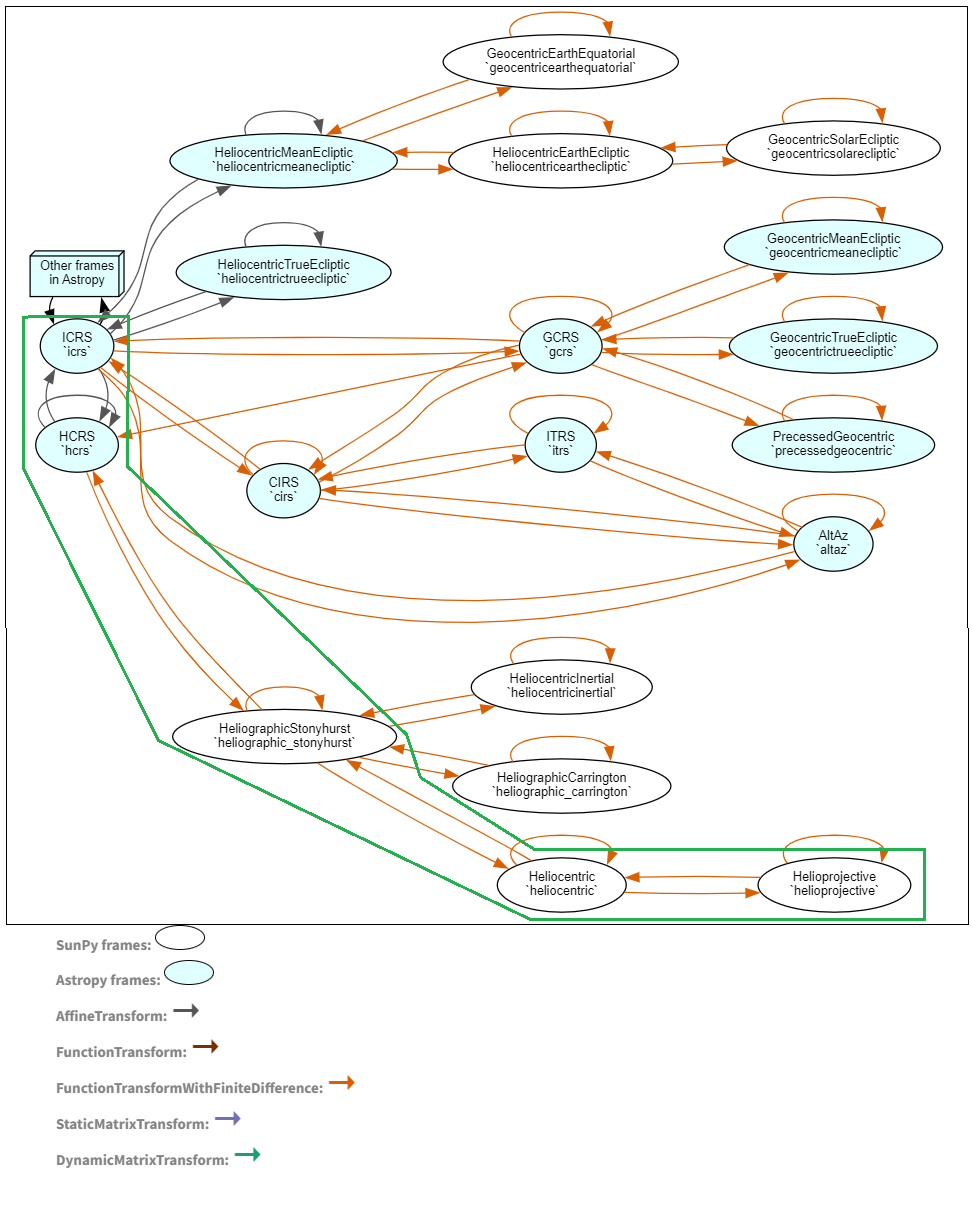
\includegraphics[width = 12cm]{report/Figures/methods/coordinates.png}
        \caption{Caption}
        \label{coordinates}
    \end{figure}

    \begin{figure}[H]
        \centering
        
\includegraphics[width = \textwidth]{report/Figures/methods/GOES_total.png}
        \caption{Caption}
        \label{goes_tot}
    \end{figure}
    